\def\CC{{C\nolinebreak[4]\hspace{-.05em}\raisebox{.4ex}{\tiny\bf ++}}}


\begin{frame}\frametitle{Outline}
\begin{itemize}
   \item Mixtures in \mirgecom (few slides ~ 5ish)
   % \item What is \pyrometheus, and what does it do (1 slide)
   % \item How is \pyrometheus{} used in \mirgecom (2 slides)
   % \begin{itemize}
   %      \item EOS
   %      \item Chemistry
   %      \item Transport?
   % \end{itemize}
   % \item \pyrometheus{} software integration into \mirgecom (5 slides)
   \item \mirgecom Performance for mixtures
   \begin{itemize}
      \item Combozzle - Bozzle with combustion, relevance
      \item \mirgecom performance of single gas NS (eager vs. lazy)
      \item Compared to mixture (eager vs. lazy)
      \item Single gas vs. mixture (eager vs. lazy)
      \item Eager is right out 
      \item Gridscaling performance
      \item Number of Newton iterations performance
      \item 
   \end{itemize}
   \item Performance goals (1-2 ish)
   \begin{itemize}
      \item 100M elements (3rd or 4th order), UIUC mixture
      \item several flowthrough's (1flowthrough $\approx$ 60us)
      \item What to expect, partitioning, communication
   \end{itemize}
\item Wrap-up (1 slide)
\end{itemize}
\end{frame}

\begin{frame}\frametitle{Mixtures with \textit{MIRGE-Euler}}
  \begin{center}
  Goal: Add reactive mixture mechanisms to \mirgecom{}\\
  Plan: Use \textit{Prometheus} / \pyrometheus\\
  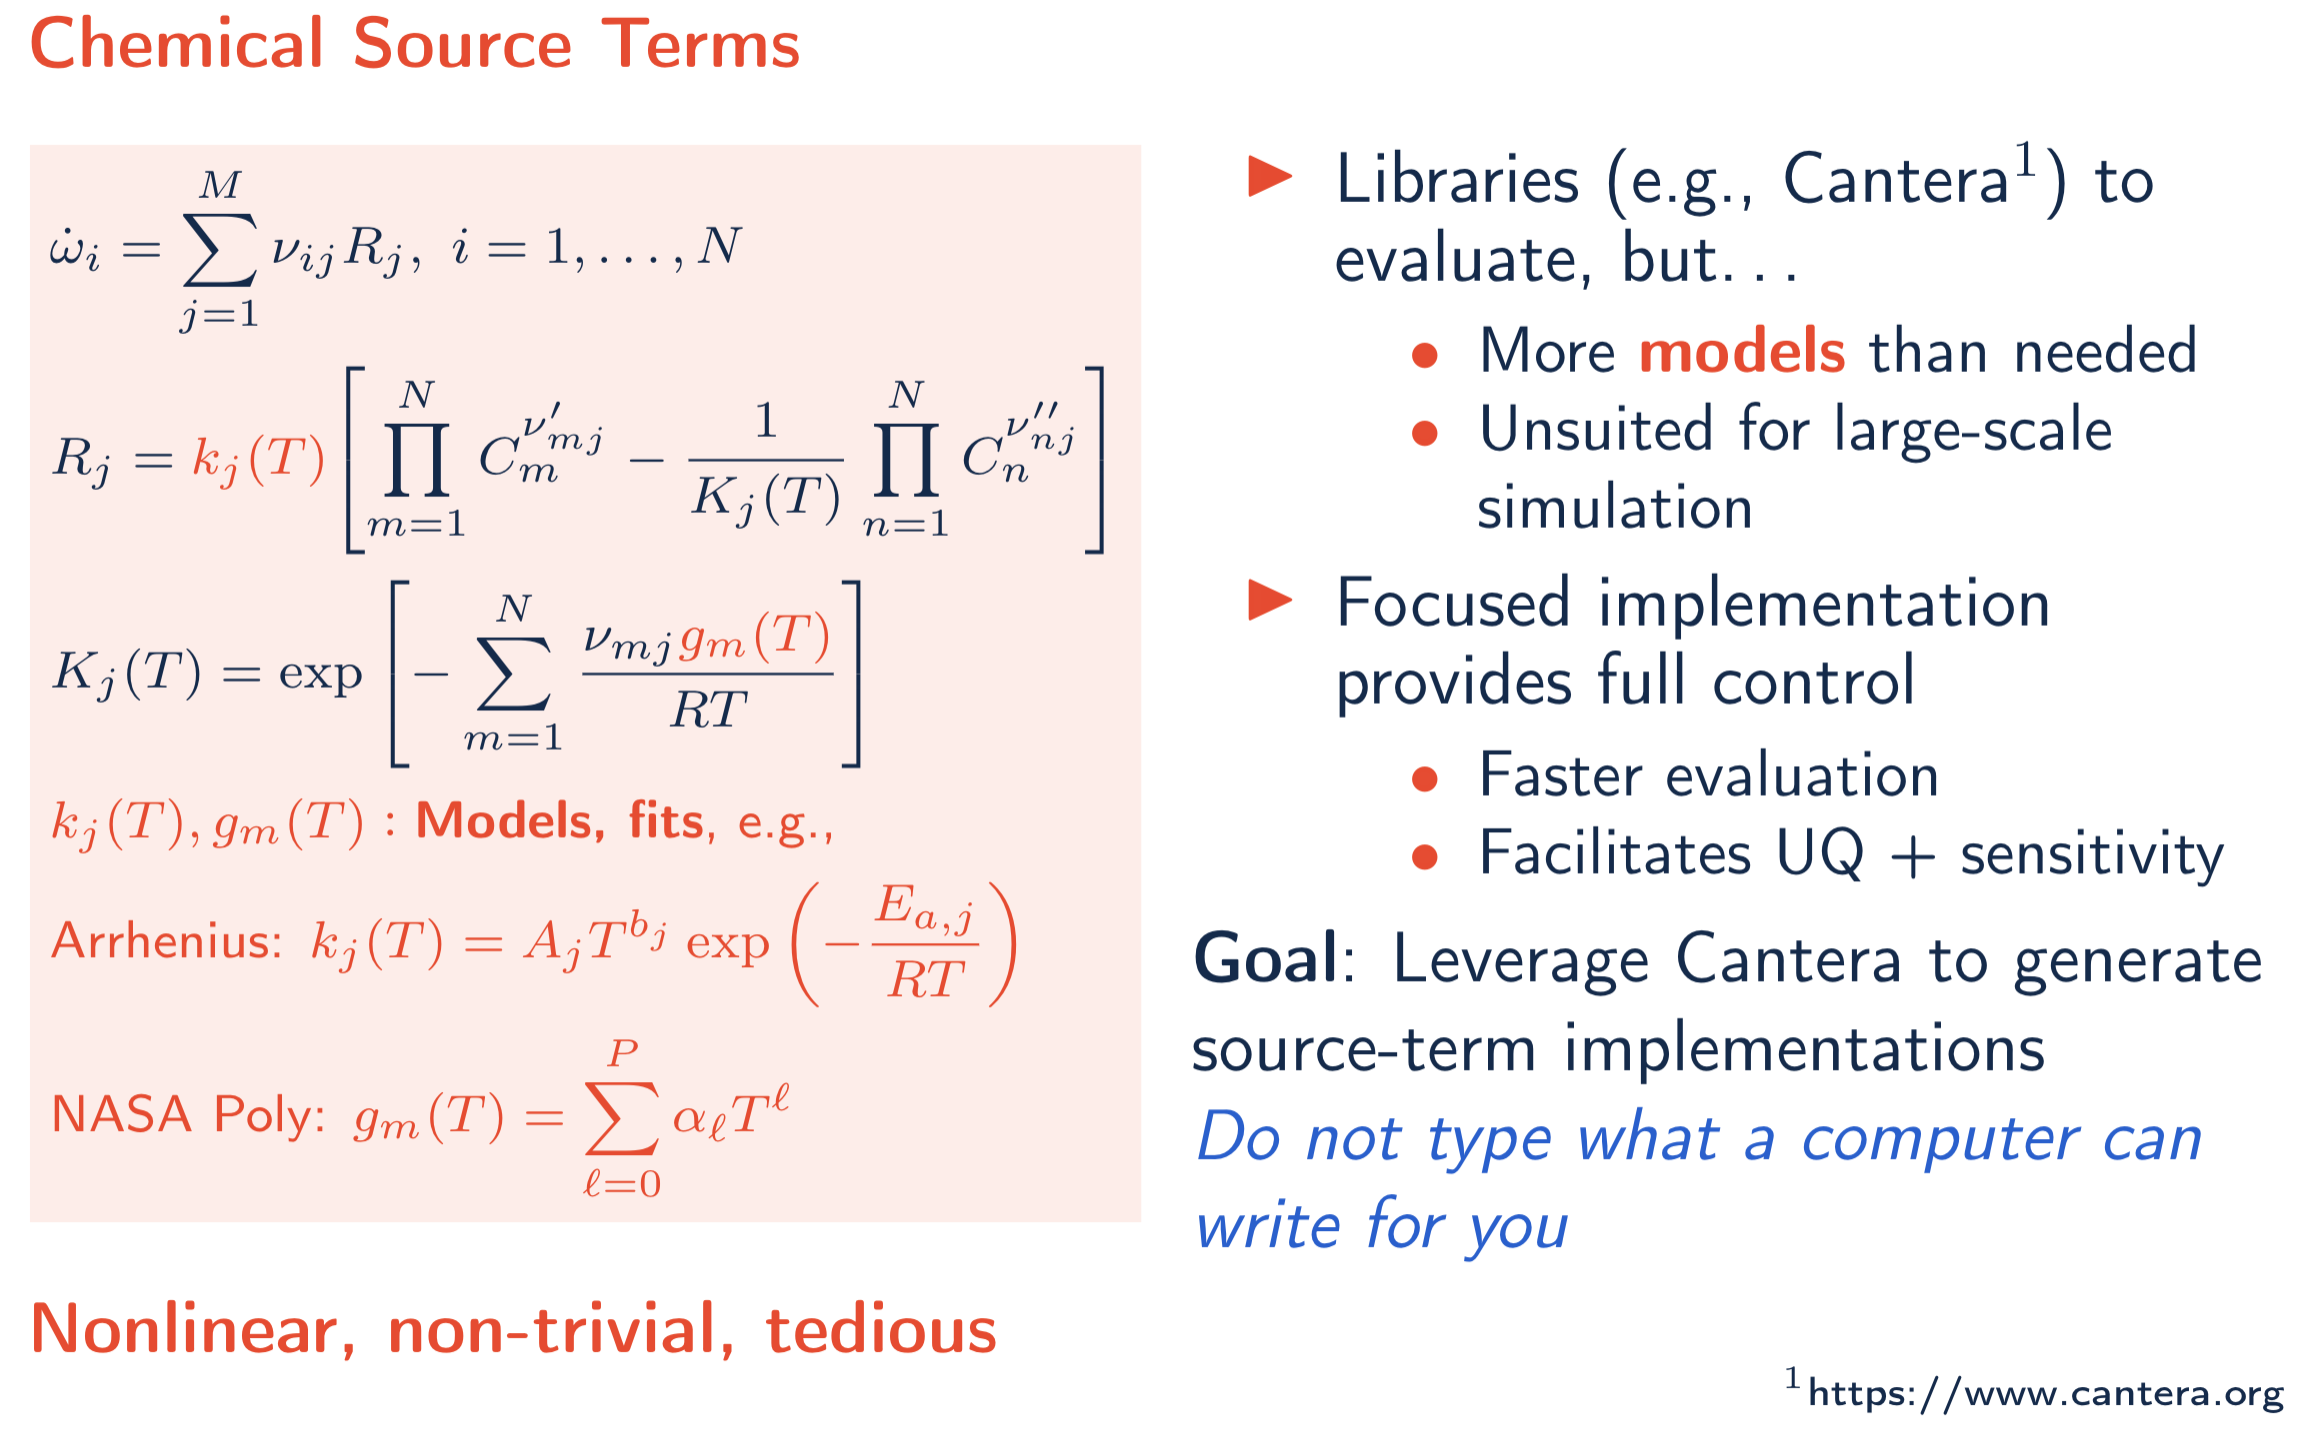
\includegraphics[width=.8\textwidth]{figures/mtc/Prometheus1.png}
  \\
 \prj{\tiny}{Esteban Cisneros}
  \end{center}
\end{frame}

\begin{frame}\frametitle{\textit{Prometheus} $\rightarrow$ \pyrometheus}
  \begin{multicols}{2}
%    \begin{itemize}
%    \item \textit{Prometheus}
      \begin{itemize}
      \item ThermoChemistry source generator (C\plusplus{})
      \item Uses \textit{Cantera} and generates C\plusplus{} or Python
      \end{itemize}
      \columnbreak
%    \item \pyrometheus
      \begin{itemize}
      \item Generator port to Python (inline)
      \item Vectorize + \textit{MIRGE}-compatible
      \item \textit{MIRGE-Euler} EOS
      \end{itemize}
%    \end{itemize}
  \end{multicols}
%  \vspace{-15pt}
  \begin{multicols}{2}
    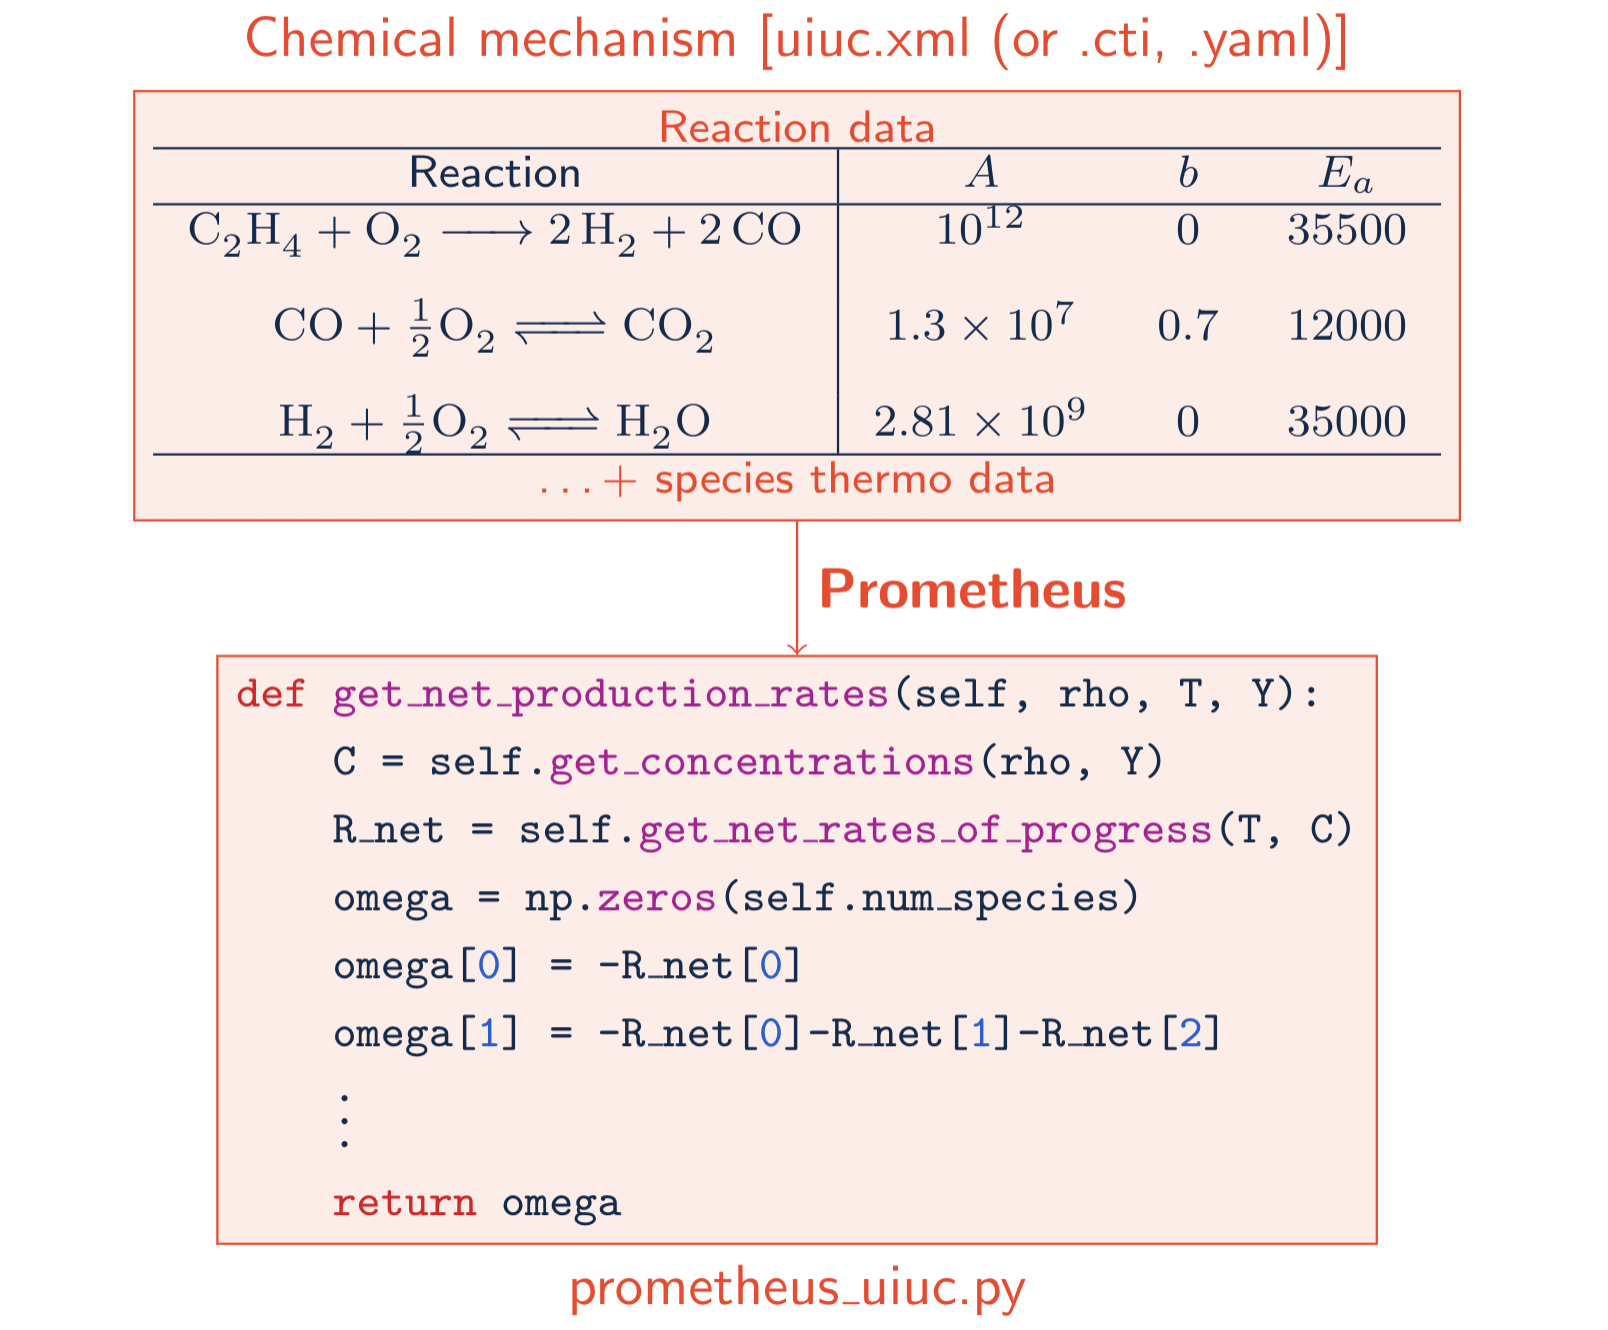
\includegraphics[width=.5\textwidth]{figures/mtc/Prometheus2.png}\\
    \begin{center}
      \prj{\tiny}{Esteban Cisneros}
    \end{center}
      \columnbreak
      \vspace{10pt}
    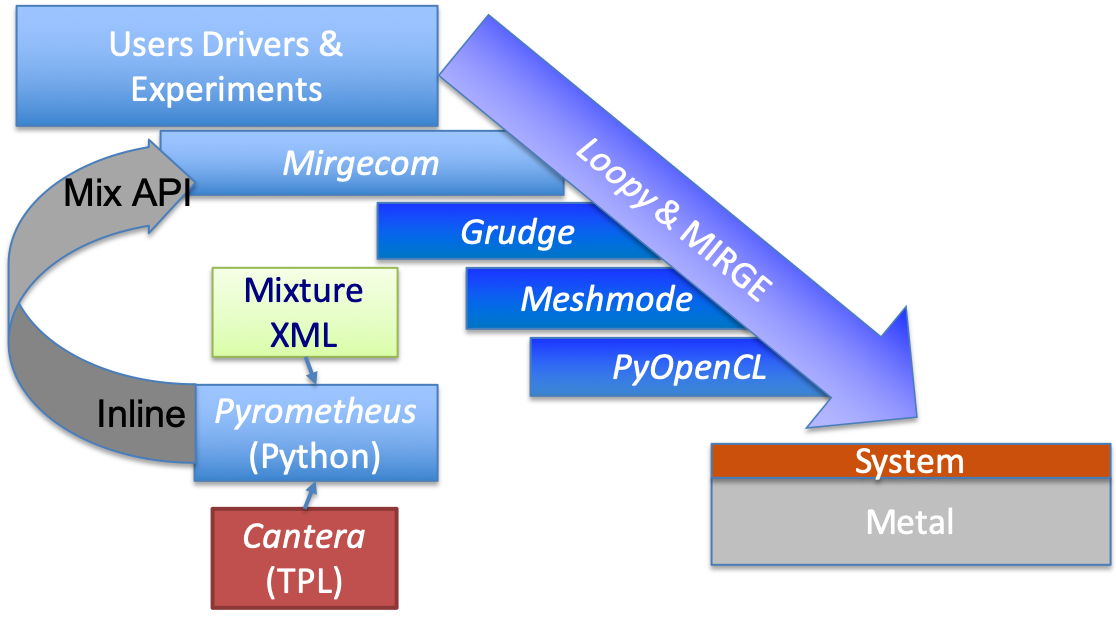
\includegraphics[width=.5\textwidth]{figures/mtc/PyrometheusIntegration.png}    
  \end{multicols}
\end{frame}

\begin{frame}\frametitle{\textit{Prometheus} mechanism code generation}
\begin{multicols}{2}
\begin{itemize}
   \item \plusplus{C} command-line utility (is not Python)
   \item XML $\rightarrow$ \textit{Prometheus}(\textit{Cantera}) $\rightarrow$ Python interface for EOS, chemistry, (\& transport)
\end{itemize}
\begin{itemize}
   \item Integration options:
   \begin{itemize}
      \item Full integration - \textit{mirgecom} ingests XML, uses \textit{Prometheus} to generate mechanism, including mechanism in \textit{mirgecom} library
      \item Partial integration - \textit{Prometheus} pre-generates mechanism for inclusion of interface into \textit{mirgecom} library
      \item Non-integration - \textit{Prometheus} stand-alone library implements one or more mechanisms and is used as a substrate library by \textit{mirgecom} 
   \end{itemize}
    \item Staged integration - partial $\rightarrow$ full
   \item Tests we can do right away (regardless of integration level):
   \begin{itemize}
      \item Pre-generated mechanism Python code inclusion (\textit{mirgecom} build and run)
      \item Pre-generated mechanism function invocations (smoke tests \& screening)
   \end{itemize}
\end{itemize}
\end{multicols}
\end{frame}

\begin{frame}\frametitle{\textit{Prometheus} EOS}
\begin{multicols}{2}
\begin{itemize}
   \item Interface functions
   \begin{itemize}
      \item get\_temperature(e, Y, Tguess) $\rightarrow (T, Cp_{mix}, R_{mix})$
      \item get\_pressure(Y, T) $\rightarrow P_{mix}$ 
      \item get\_mix\_cp(T, Y) $\rightarrow (Cp_{mix})$ 
      \item get\_mix\_cv(T, Y) $\rightarrow (Cv_{mix})$
      \item get\_mix\_e(T, Y) $\rightarrow (e)$
      \item get\_mix\_enthalpy(T, Y) $\rightarrow (h_{mix})$
      \item get\_species\_cp\_R(T) $\rightarrow (Cp_{i})$ 
      \item get\_species\_enthalpies(T, Y) $\rightarrow (h_{i})$
   \end{itemize}
   \item Wrap interface to \textit{mirgecom} standard EOS - small to medium effort
   \item Special considerations
   \begin{itemize}
      \item Species ordering, naming
      \item Buffer species handling
   \end{itemize}
   \item Potential tests:
   \begin{itemize}
     \item Species-specific mixture tests (i.e. one species-at-a-time)
     \item Calorically perfect mixture - Compare Prometheus vs. \textit{mirgecom}@CPEOS
     \item Thermally perfect mixture with linear $Cp_i$ - test temperature inversion vs. analytic? 
   \end{itemize}
\end{itemize}
\end{multicols}
\end{frame}

\begin{frame}\frametitle{Wrappers for \textit{Prometheus} EOS}
Create \textit{mirgecom}-EOS-compatible wrappers for \textit{Prometheus} interface functions.
\begin{itemize}
\item get\_pressure(state)
\item get\_temperature(state)
\item get\_internal\_energy(state)
\item get\_speed\_of\_sound(state)
\end{itemize}
\end{frame}

\begin{frame}\frametitle{\textit{Prometheus} chemistry \& transport}
\begin{itemize}
\item Chemistry - get\_net\_production\_rates($\rho$, T, Y) $\rightarrow (\dot{\omega}_i)$
\item For explicit integration - directly feeds species source terms $S_i = (W_i \dot{\omega}_i)$
\item Transport
   \begin{itemize}
      \item Species:  $(\kappa_i, \mu_i, D_{ij})$
      \item Mixture: $(\kappa, \mu, D_i)$
   \end{itemize}
\end{itemize}
%\end{multicols}
\end{frame}

\begin{frame}\frametitle{Integrating \textit{Prometheus} into \textit{mirgecom}}
There are 4 \textit{Prometheus} constructs to consider for integration:
\begin{itemize}
\item Mechanism generation
\item Equation of state (EOS)
\item Chemistry
\item ``Advanced'' transport (future)
\end{itemize}
\end{frame}


\begin{frame}\frametitle{\textit{Prometheus} / \textit{mirgecom} wishlist}
\begin{itemize}
   \item get\_species\_index(species\_name) - useful for coding the interface/wrappers
   \item get\_species\_names - for I/O, viz/analysis
\end{itemize}           
\end{frame}


% \begin{frame}\frametitle{MIRGE Overview}
% 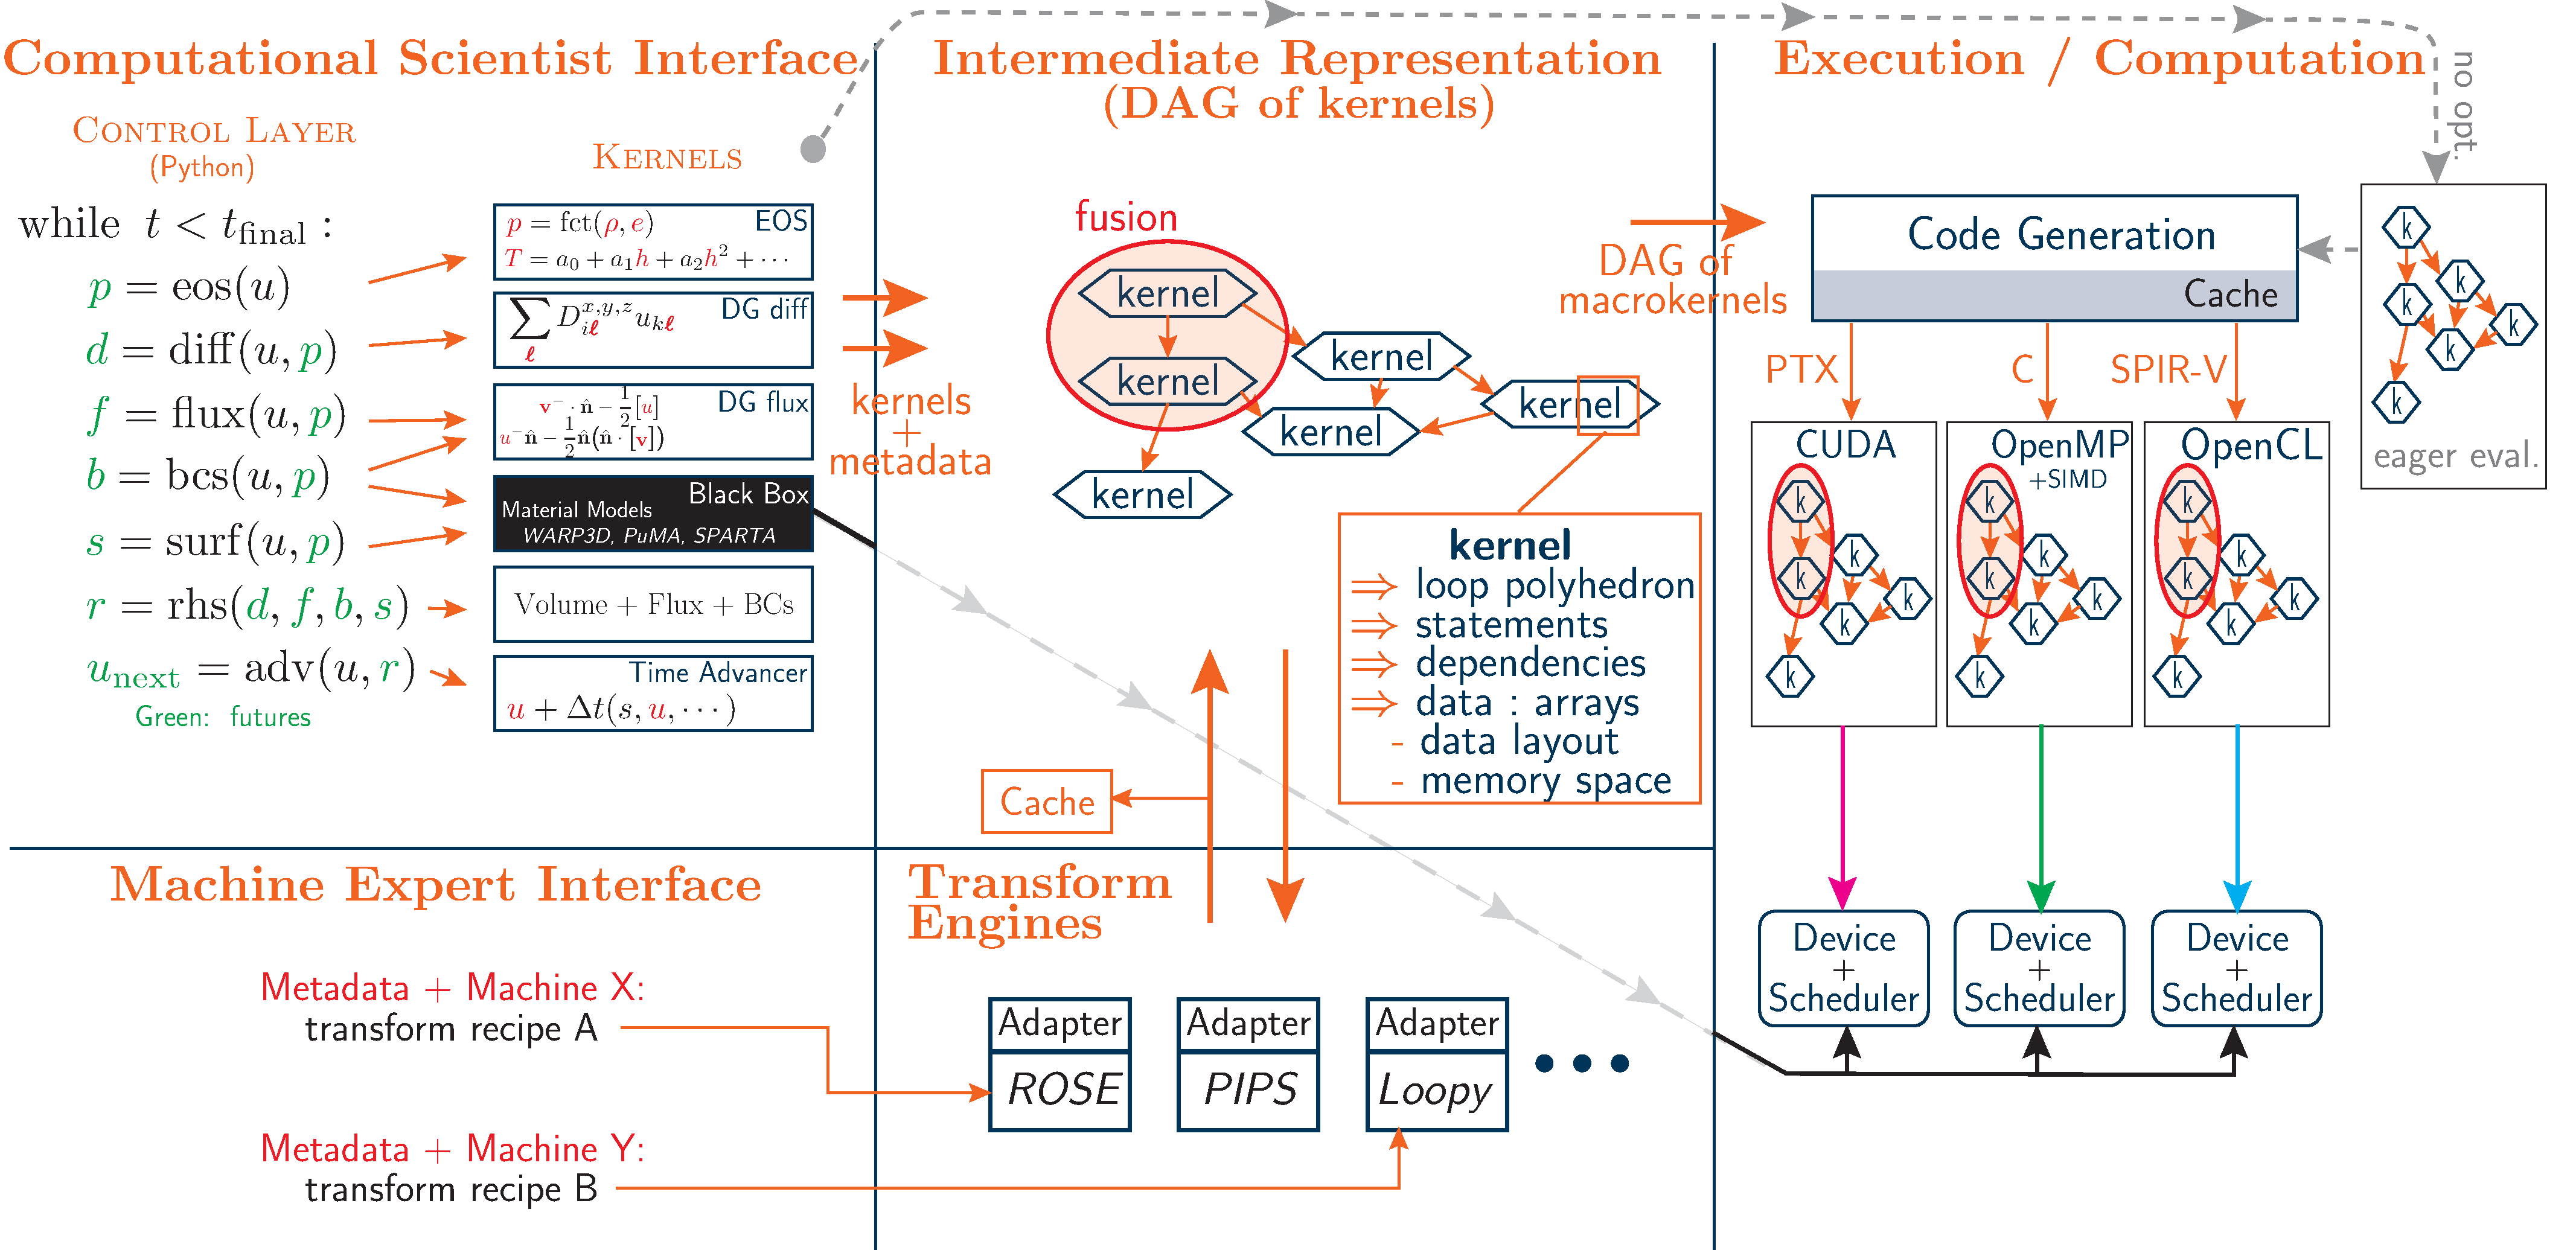
\includegraphics[width=\textwidth]{../01-Overview/figures/controllayer-new.pdf}
% \end{frame}




\begin{frame}\frametitle{Navier-Stokes with combustion sources}
  \begin{center}
  %Evolution equation:
  %Governing equation is Navier--Stokes:
  \begin{equation*}
    \frac{\partial\mathbf{Q}}{\partial{t}} + \nabla \cdot (\mathbf{F}^I - \mathbf{F}^V) - \mathbf{S} = 0
  \end{equation*}
  % With chemistry source terms:
  % \begin{equation*}
  %  \mathbf{S} = [ 0, 0, 0, 0, 0, W_k\dot{\omega_k} ]
  %\end{equation*}
    Where state vector $\mathbf{Q}$, fluxes $\mathbf{F}^I$, $\mathbf{F}^V$ , and sources $\mathbf{S}$ are given by:
 \begin{equation*}
      \begin{bmatrix}
        \rho\\\rho{E}\\\rho\vec{v}\\\rho{Y}_\alpha\end{bmatrix},\quad
      \begin{bmatrix} \rho\vec{v}\\(\rho{E} +
        p)\vec{v}\\\rho(\vec{v} \otimes \vec{v}) +
        p\delta_{ij}\\\rho{Y}_\alpha\vec{v}\end{bmatrix}, \quad
       \begin{bmatrix} 0\\(\mathbf{\tau} \cdot \vec{v} - \mathbf{q})\\\mathbf{\tau}_{:j}\\-\mathbf{J}_\alpha\end{bmatrix},\quad
       \begin{bmatrix} 0\\0\\0\\W_\alpha\dot{\omega}_\alpha\end{bmatrix},
 \end{equation*}
with $\tau = \mu\left(\nabla\vec{v} - \nabla\vec{v}^T\right) + \left(\mu_b - \frac{2\mu}{3}\right)\left(\nabla \cdot \vec{v}\right)$,\\
\vspace{5pt}
$\mathbf{J}_\alpha = -\rho d_{(\alpha)} \nabla(Y_\alpha)$, and $\mathbf{q} = -\kappa\nabla{T}$\\
\vspace{10pt}
    The mixture gas model (EOS) provides $\rightarrow~~(p,T,e,\mu,\kappa,d_{\alpha}, \omega_\alpha)(\mathbf{Q})$
  \end{center}
\end{frame}


% AK-sanctioned rip-off 
% \begin{frame}\frametitle{DG - The program}
%   \begin{multicols}{2}
%     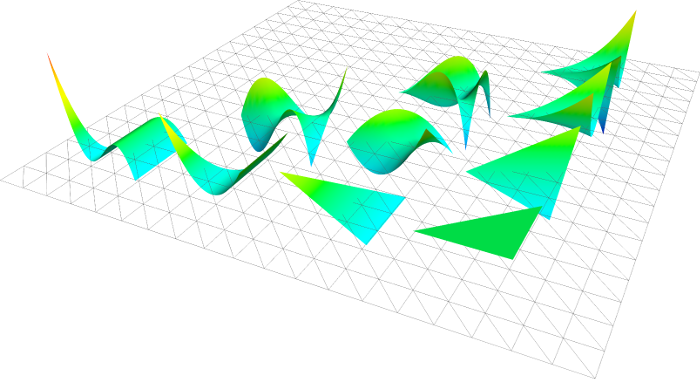
\includegraphics[width=0.4\textwidth]{../02-CS/Figures/pkdo-2d.png}
%     \vspace{-10pt}
%    \newcommand{\meshnodes}{
  \coordinate (a) at (4.53,2.86) ;
  \coordinate (b) at (2.91,3.55) ;
  \coordinate (c) at (2.25,1.8) ;
  \coordinate (d) at (-0.3,3.25) ;
  \coordinate (e) at (1.31,4.17) ;
  \coordinate (f) at (1.19,0.43) ;
  \coordinate (g) at (2.77,0.7) ;
  \coordinate (h) at (3.96,3.54) ;
  \coordinate (i) at (0.05,1.17) ;
  \coordinate (j) at (2,3.1) ;
  \coordinate (k) at (3,4.7) ;
  \coordinate (m) at (3.93,1.65) ;
  \coordinate (n) at (1.78,0.76) ;
  \coordinate (o) at (0.40,4.4) ;
  \coordinate (p) at (0.8,2.5) ;
  \coordinate (q) at (4.72,1.32) ;
  \coordinate (r) at (3.02,2.27) ;
  \coordinate (s) at (0.98,1.83) ;
  \coordinate (t) at (-0.3,1.8) ;
}


\newcommand{\withmeshtris}[1]{
  #1 cgn #1 snf #1 jsc #1 pjs
  #1 pts #1 sif #1 sit #1 dtp
  #1 odp #1 epj #1 jcb #1 oep
  #1 rcg #1 crb #1 kbh #1 rah
  #1 ejb #1 rgm #1 ram #1 qam
  #1 ekb #1 gqm #1 scn #1 bhr
}

\newcommand{\drawtriangle}[3]
  {\draw (#1) -- (#2) -- (#3) -- cycle;}
\newcommand{\meshtris}{
  \withmeshtris\drawtriangle
}
\def\drawnodenames{
  \foreach \i in {a,b,c,d,e,f,g,h,i,j,k,m,n,o,p,q,r,s,t}
    \node at (\i) {\i};
}
  

%     \begin{tikzpicture}[scale=0.4]
%       \meshnodes
%       \meshtris
%       \draw [fill=blue!30] (c) -- (n) -- (g) ;
%       \node [left=10mm of g,xshift=-2mm] (ellabel) {$E_k$};
%       \draw [thick,->,shorten >=2mm] (ellabel) -- (c) ;
%     \end{tikzpicture}
%     \vspace{-10pt}
%     \prj{\tiny}{Kl{\"o}ckner}\columnbreak \\
%     Numerical approximation to $\mathbf{Q}$, $\mathbf{S}$:
%     \begin{equation*}
%       \partial_t\mathbf{q}^{*} + \nabla \cdot \mathbf{F}(\mathbf{q}^{*}) - \mathbf{s}^{*} = 0
%     \end{equation*}
%     Hit with test function and integrate over element:
%     \begin{equation*}
%       \int_{E_k}[(\partial_t\mathbf{q}^{*} - \mathbf{s}^{*}) + (\nabla \cdot \mathbf{F}(\mathbf{q}^{*}))]\phi\,dx = 0
%     \end{equation*}
%   \end{multicols}
 %  \begin{center}
%     Integrate by parts:
%     \begin{equation*}
%       \int_{E_k}(\partial_t\mathbf{q}^{*}- \mathbf{s}^{*})\phi\,dx -
%       \int_{E_k}(\mathbf{F}(\mathbf{q}^{*}) \cdot \nabla{\phi})\,dx +
%       \int_{\partial{E_k}}(\hat{n} \cdot \mathbf{F}(\mathbf{q}^{*}))\phi\,dx
%     \end{equation*}
 %  \end{center}
%   \begin{center}
%     Rearranging in matrix form:
%     \begin{equation*}
%       \mathcal{M}[\partial_t\mathbf{q}^{*}] = \mathcal{M}[\mathbf{s}^{*}] + ( \mathcal{S}[\mathbf{F}(\mathbf{q}^{*})] )
%       - \sum{\mathcal{M}_{\partial{E_k}}[(\hat{\mathbf{n}} \cdot \mathbf{f}^{*})]} ) 
%     \end{equation*}
%   \end{center}
% \end{frame}



%\begin{frame}\frametitle{Example Euler simulation applications}
%\begin{multicols}{2}
%  \begin{itemize}
%  \item CI-exercised verification cases 
%    \begin{itemize}
%    \item Isentropic vortex
%    \item Sod's shock
%    \item Scalar advection
%    \end{itemize}
%  \item More simulation support stuff
%    \begin{itemize}
%    \item Grid gen/decomp (serial)
%    \item Generic time marching
%    \item RK4 time integrator 
%    \item Viz I/O - VTK file/process
%    \item Status \& profiling \prj{\tiny}{M.~Diener}
%    \end{itemize}
%\end{itemize}
%\end{multicols}
%\begin{multicols}{2}
%  \lstinputlisting[style=kkcodestyle, basicstyle=\tiny, language=Python]{figures/mtc/vortex_driver.py}
%  \lstinputlisting[style=kkcodestyle, basicstyle=\tiny, language=Python]{figures/mtc/vortex_driver1.py}
%  \columnbreak
%  \lstinputlisting[style=kkcodestyle, basicstyle=\tiny, language=Python]{figures/mtc/vortex_driver2.py}
%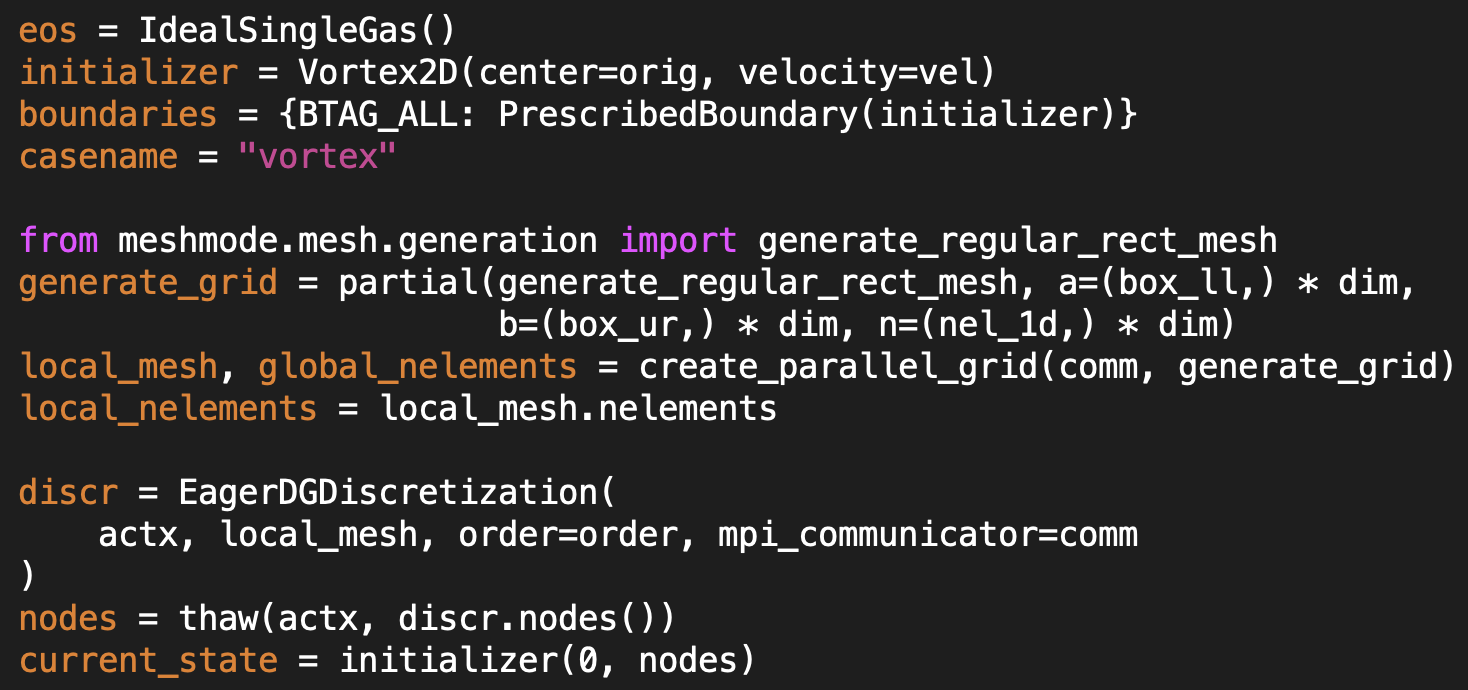
\includegraphics[width=.45\textwidth]{figures/mtc/vortex_driver1.py}
%\hspace{.2in}
%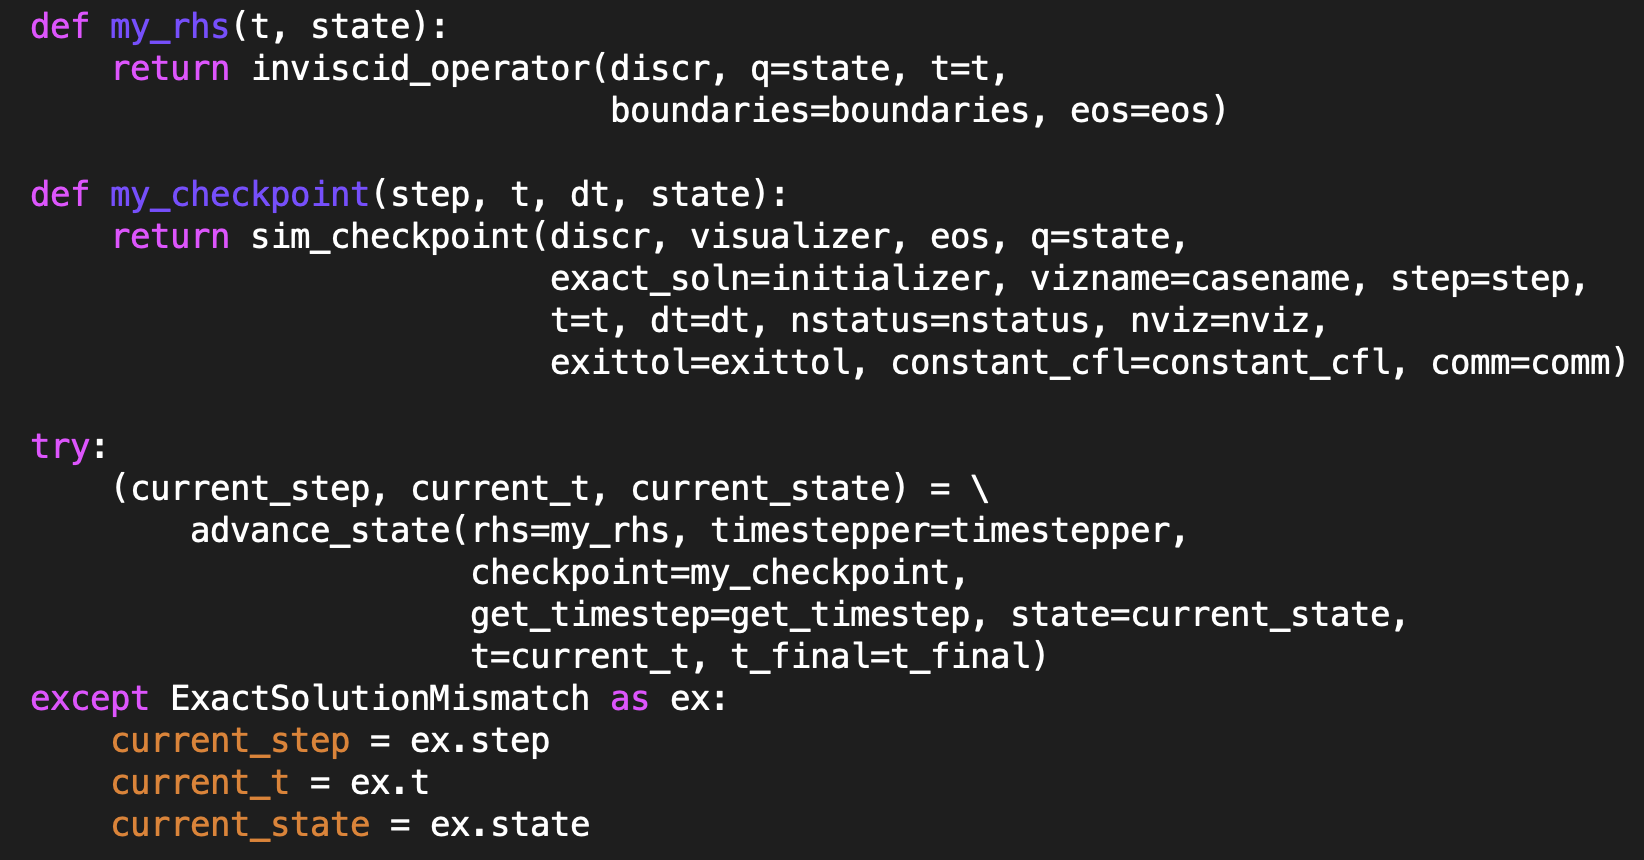
\includegraphics[width=.45\textwidth]{figures/mtc/vortex_driver2.py}
%\end{multicols}
%\end{frame}


%\begin{frame}\frametitle{\textit{Pyrometheus} integration with \textit{MIRGE-Euler}}
%    \begin{multicols}{2}
%    \begin{itemize}
%    \item Port \textit{Prometheus} generator to Python $\rightarrow$ \textit{Pyrometheus}
%    \item Massage interface for MIRGE paradigm
%    \item Implement EOS and Chem Source
%    \end{itemize}
%    \end{multicols}
%    \begin{multicols}{2}
%      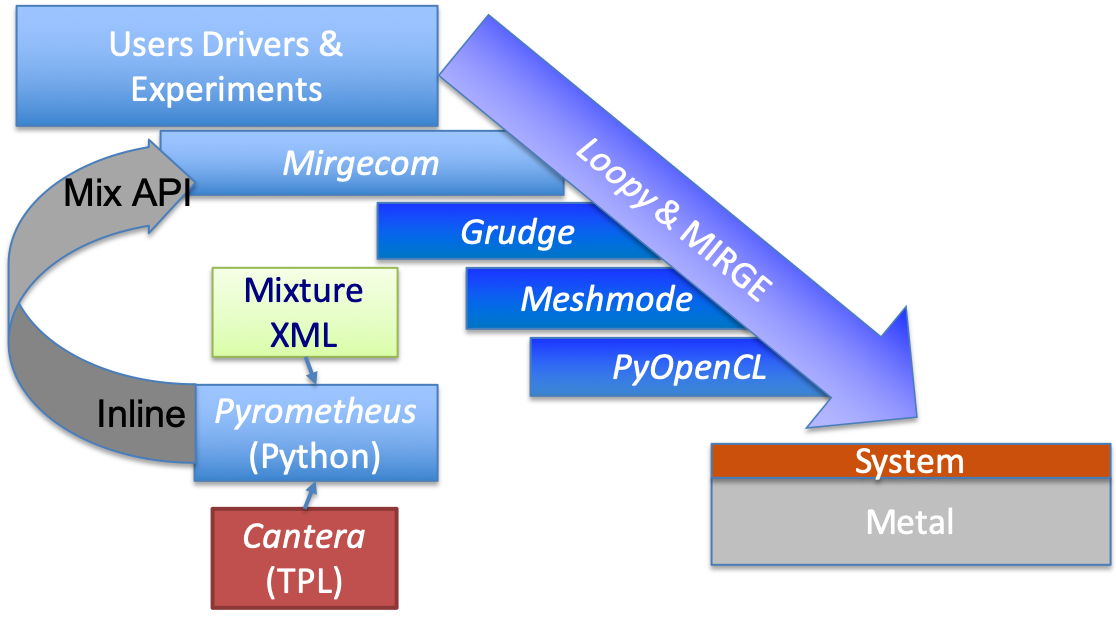
\includegraphics[width=.5\textwidth]{figures/mtc/PyrometheusIntegration.png}\\
%      \columnbreak
%      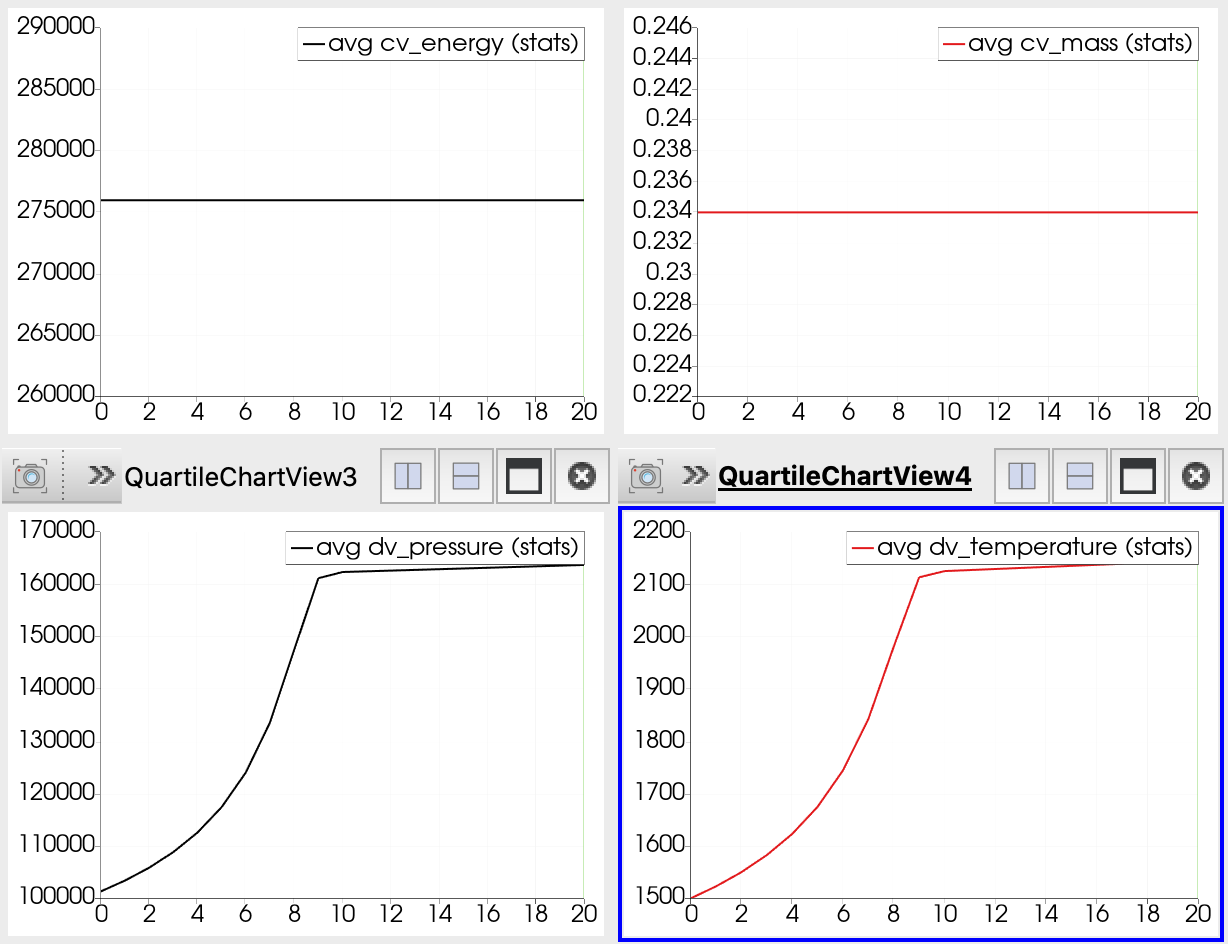
\includegraphics[width=.5\textwidth]{figures/mtc/autoignition_data_raw.png}
%     \end{multicols}
%\end{frame}

\begin{frame}\frametitle{\pyrometheus in \textit{MIRGE-Euler}}
  \begin{multicols}{2}
    Governing equation is Navier--Stokes:
    \begin{equation*}
      \frac{\partial\mathbf{Q}}{\partial{t}} + \nabla \cdot (\mathbf{F}^I - \mathbf{F}^V) - \mathbf{S} = 0
    \end{equation*}
    With chemistry source terms:
    \begin{equation*}
      \mathbf{S} = [ 0, 0, 0, 0, 0, W_k\dot{\omega_k} ]
    \end{equation*}
    Thermo state functions:
    \begin{equation*}
      (p, T, e_k) = f(\mathbf{Q})
    \end{equation*}
    \begin{center}
      \prj{\tiny}{\textit{Prometheus} documentation}
    \end{center}
    \columnbreak
    % \lstinputlisting[style=kkcodestyle, basicstyle=\tiny, language=Python]{figures/mtc/chemsrc.py}
  \end{multicols}
\end{frame}

\begin{frame}\frametitle{Autoignition using \textit{MIRGE-Euler}}
  \begin{multicols}{2}
    \begin{itemize}
      \item Ethylene, oxygen mixture $\phi=1$, fixed $\rho$
      \item $(p, T) = (1 \mathtt{atm}, 1500 \mathtt{K})$
      \item \textit{Prometheus}-predicted profiles match \textit{Cantera}
      \item \textit{MIRGE-Euler} co-verification w/\pyrometheus EOS
    \end{itemize}
  \end{multicols}
  \begin{multicols}{2}
    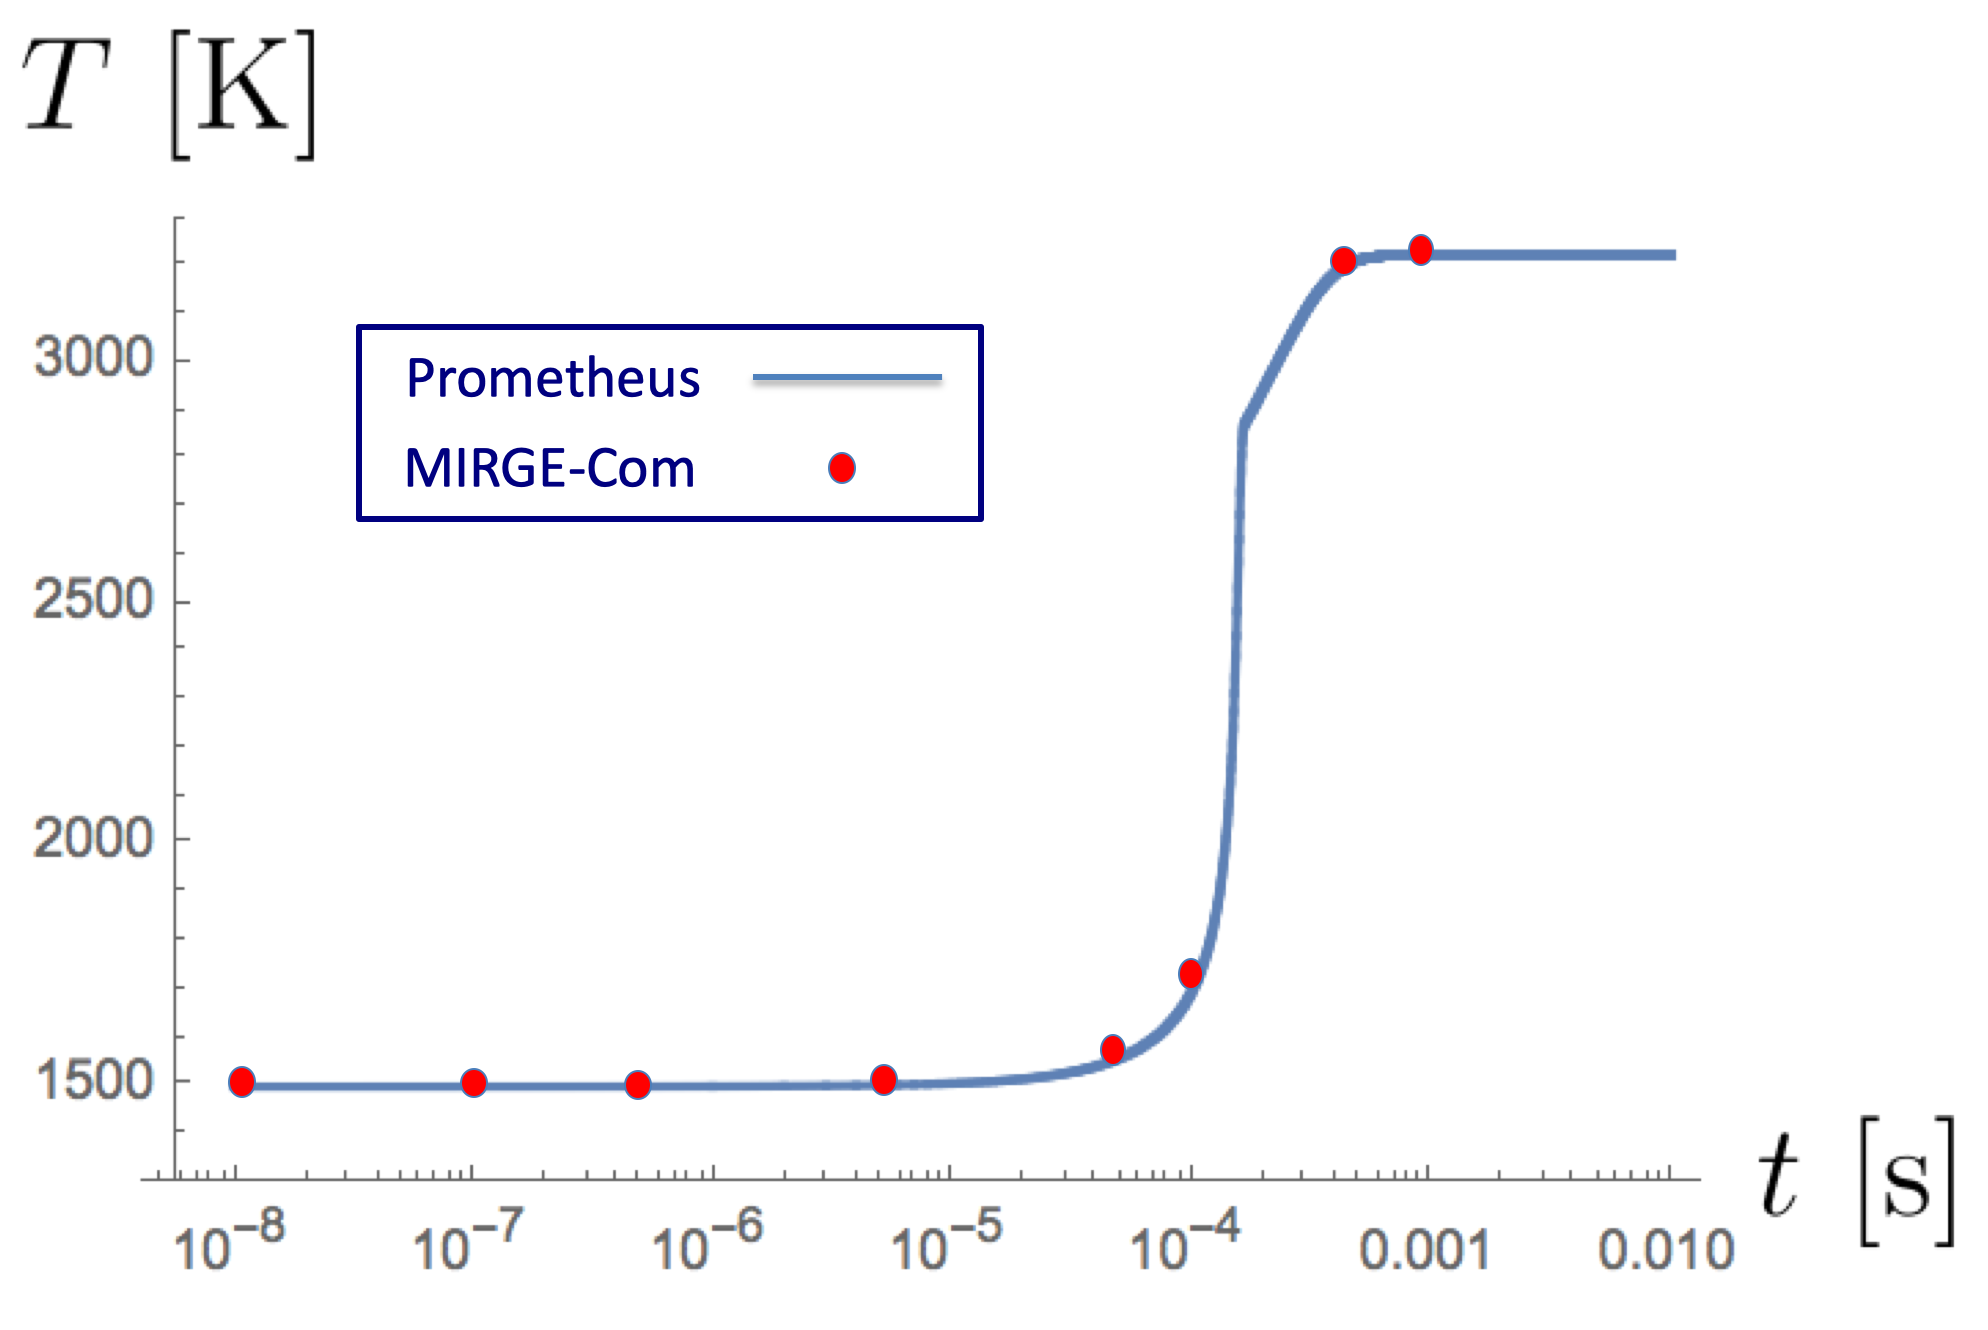
\includegraphics[width=.5\textwidth]{figures/mtc/AutoIgnition_Sudden.png}\\
    \columnbreak
    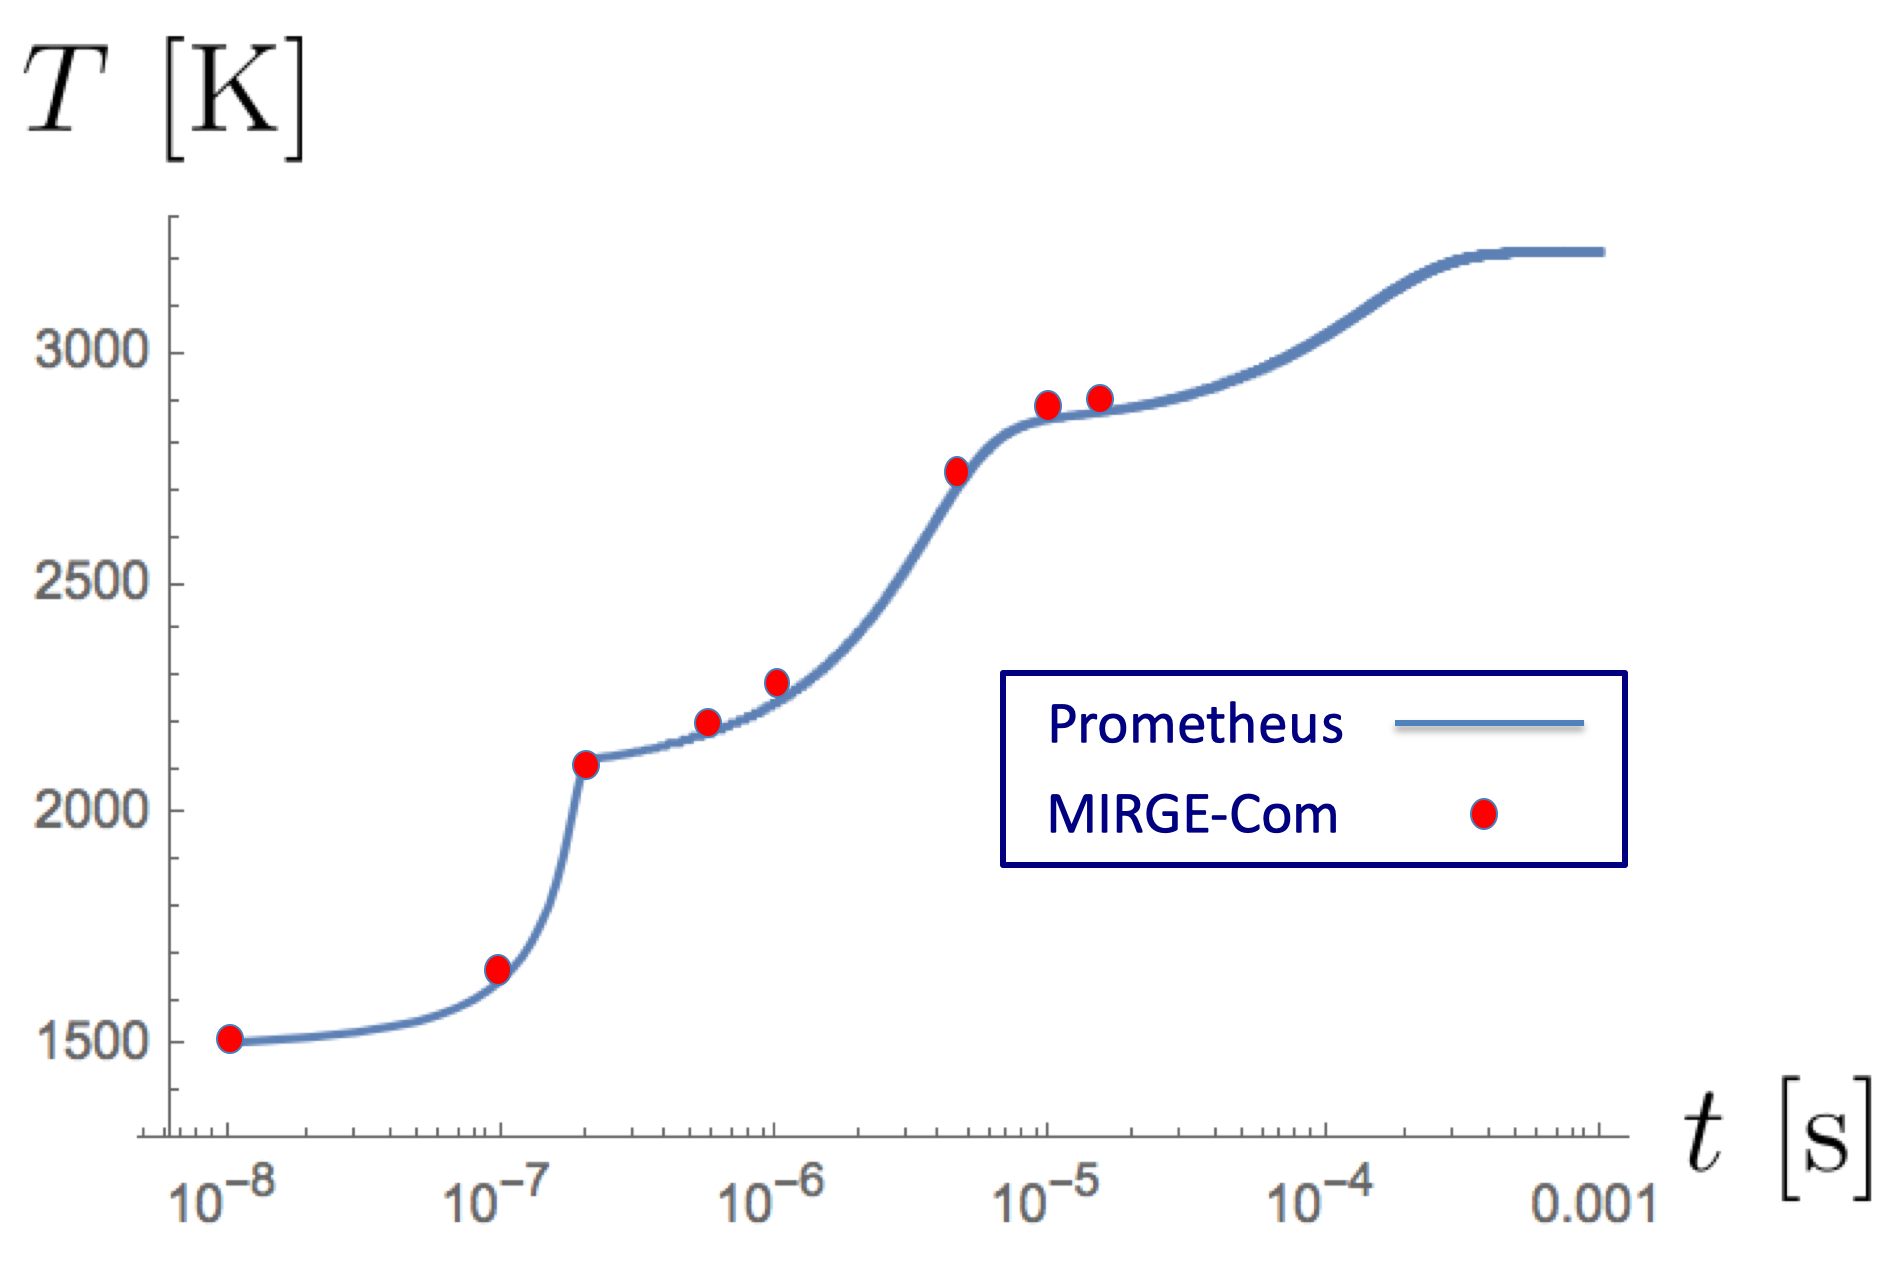
\includegraphics[width=.5\textwidth]{figures/mtc/AutoIgnition_Episodic.png}
  \end{multicols}
\end{frame}

\begin{frame}\frametitle{Retrospection \& path forward}
  \begin{multicols}{2}
    \begin{itemize}
    \item Awesome
      \begin{itemize}
        % PROS
        % 
        % - GPUs, MPI, DG
        % Very easy to go from concept and model to working simulation
      \item Follow the rules, everything works great! (GPU, MPI, DG)
      \item Easy to go from concept/model to working sim application
      \item Quite easy to read and understand 
      \item Close to the symbolic expressions
      \end{itemize}
      \columnbreak
    \item Troublesome
      \begin{itemize}
      \item Discovering the rules can be challenging
      \item Fixing things once you've run afoul of the rules
      \item Data structures are multi-faceted and can be confusing
      \item Performance is concerning
      \end{itemize}
    \end{itemize}
  \end{multicols}
  % Far more excited than frightened!
  \begin{center}
    Next for \textit{MIRGE-Com}
  \end{center}
  \begin{multicols}{2}
    \begin{itemize}
    \item Performance evaluation \& analysis \prj{\tiny}{M.~Diener}
    \item Viscous terms / Navier--Stokes / Diffusion
    \item Shock capturing \prj{\tiny}{Wyatt Hagen}
    \item Wall modeling / coupling \prj{\tiny}{M.~Smith}
    \item Post-diction in-tandem! \prj{\tiny}{M.~Anderson}
    \end{itemize}
  \end{multicols}
\end{frame}


\begin{frame}\frametitle{Daily ASC platform tests}
  %    \vspace{0pt}
  \setlength{\columnsep}{-7.0cm}
  \begin{multicols}{2}
    \begin{minipage}{.2\textwidth}
      \vspace{1cm}
      \hspace{-2cm}
    \begin{itemize}
    \item Lassen GPUs%\hspace{-2cm}%
    \item 1(+) times daily cron
    \item Exercises nozzle, 1dflame
    \end{itemize}
    \end{minipage}
    \columnbreak
    \hspace{-80pt}
    \begin{figure}[htpb]
      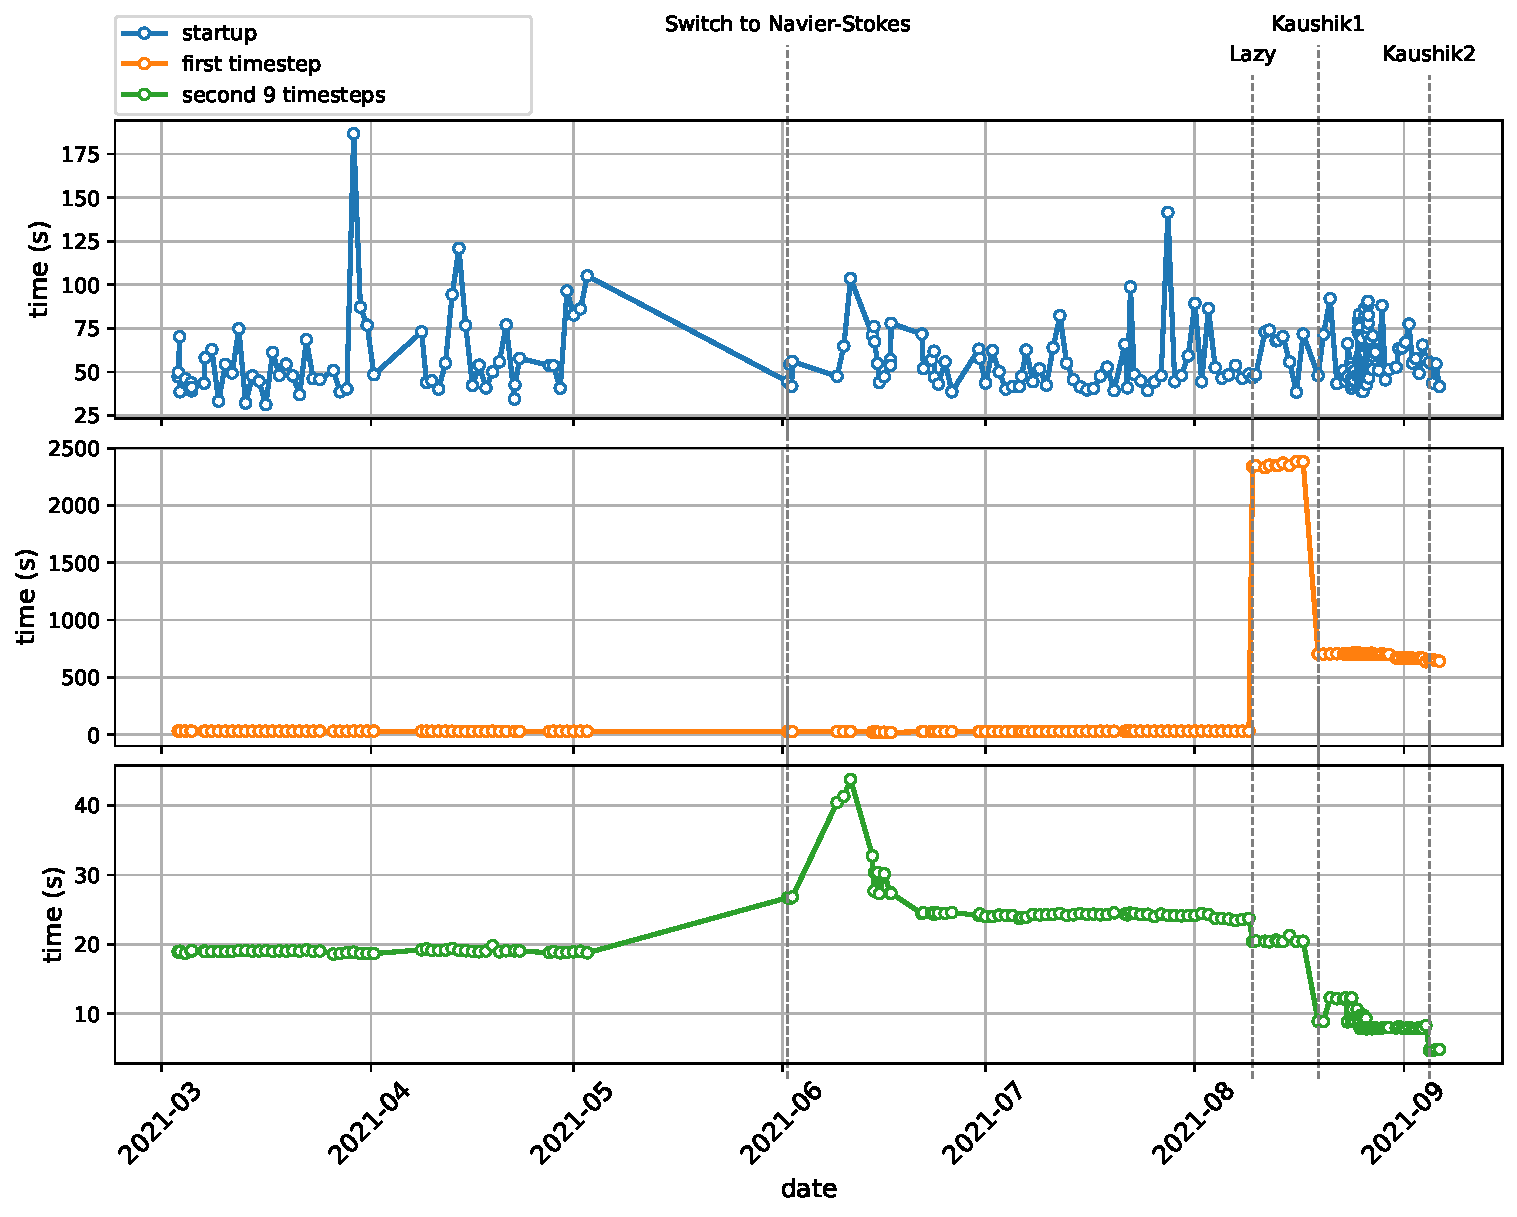
\includegraphics[width=.8\textwidth]{figures/nozzle_timing_full.pdf}
    \end{figure}		
  \end{multicols}
  \vspace{0pt}
  \begin{tikzpicture}[remember picture, overlay]
    \fill <2> [fill=white, opacity=0.8] (current page.south west) + (0.5,0.5) rectangle (12.5,9);
    \node <2> [inner sep=0pt] at (current page.center) {
      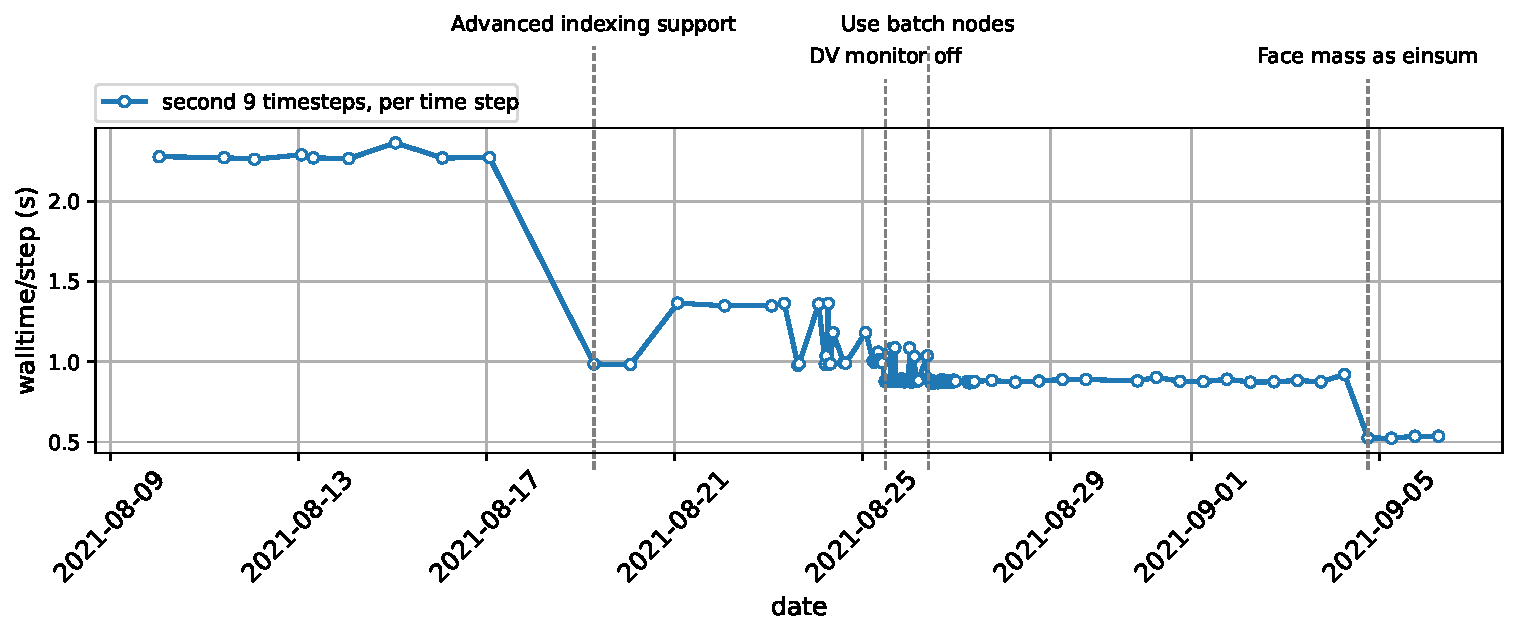
\includegraphics[width=\textwidth]{figures/nozzle_timing_detail.pdf}
    };
  \end{tikzpicture}
  % make a grid:
  % \tikz[overlay, remember picture, help lines]{
  %   \foreach \x in {0,...,12} \path (current page.south west) +(\x,9.25) node {\small$\x$};
  %   \foreach \y in {0,...,9} \path (current page.south west) +(12.5,\y) node {\small$\y$};
  %   \foreach \x in {0,0.5,...,12.5} \draw (current page.south west) ++(\x,0) -- +(0,9.6);
  %   \foreach \y in {0,0.5,...,9.5} \draw (current page.south west) ++(0,\y) -- +(12.8,0);
  % }
  %
\end{frame}

%\begin{frame}\frametitle{MIRGE-Com development environment}
%  \begin{itemize}
%  \item development process/env
%  \item user/developer support
%  \item production support (y1-production)
%  \item testing: unit, integrated, verification/regression, production, nightly timings
%  \end{itemize}
%\end{frame}

% MIRGE performance stuff
\begin{frame}\frametitle{Combozzle: scalable test case}
  \begin{minipage}{0.45\textwidth}		
    \begin{itemize}
    \item Y2-representative physics and performance in a scalable box
    \item Scaling investigations: grid, parallel, {$p$, $h$}-refinements
    \item Lazy development
    \item Performance modeling
    \item Pre-production test runs
    \end{itemize}
  \end{minipage}
  \begin{minipage}{0.5\textwidth}
    \begin{figure}
      \centering
      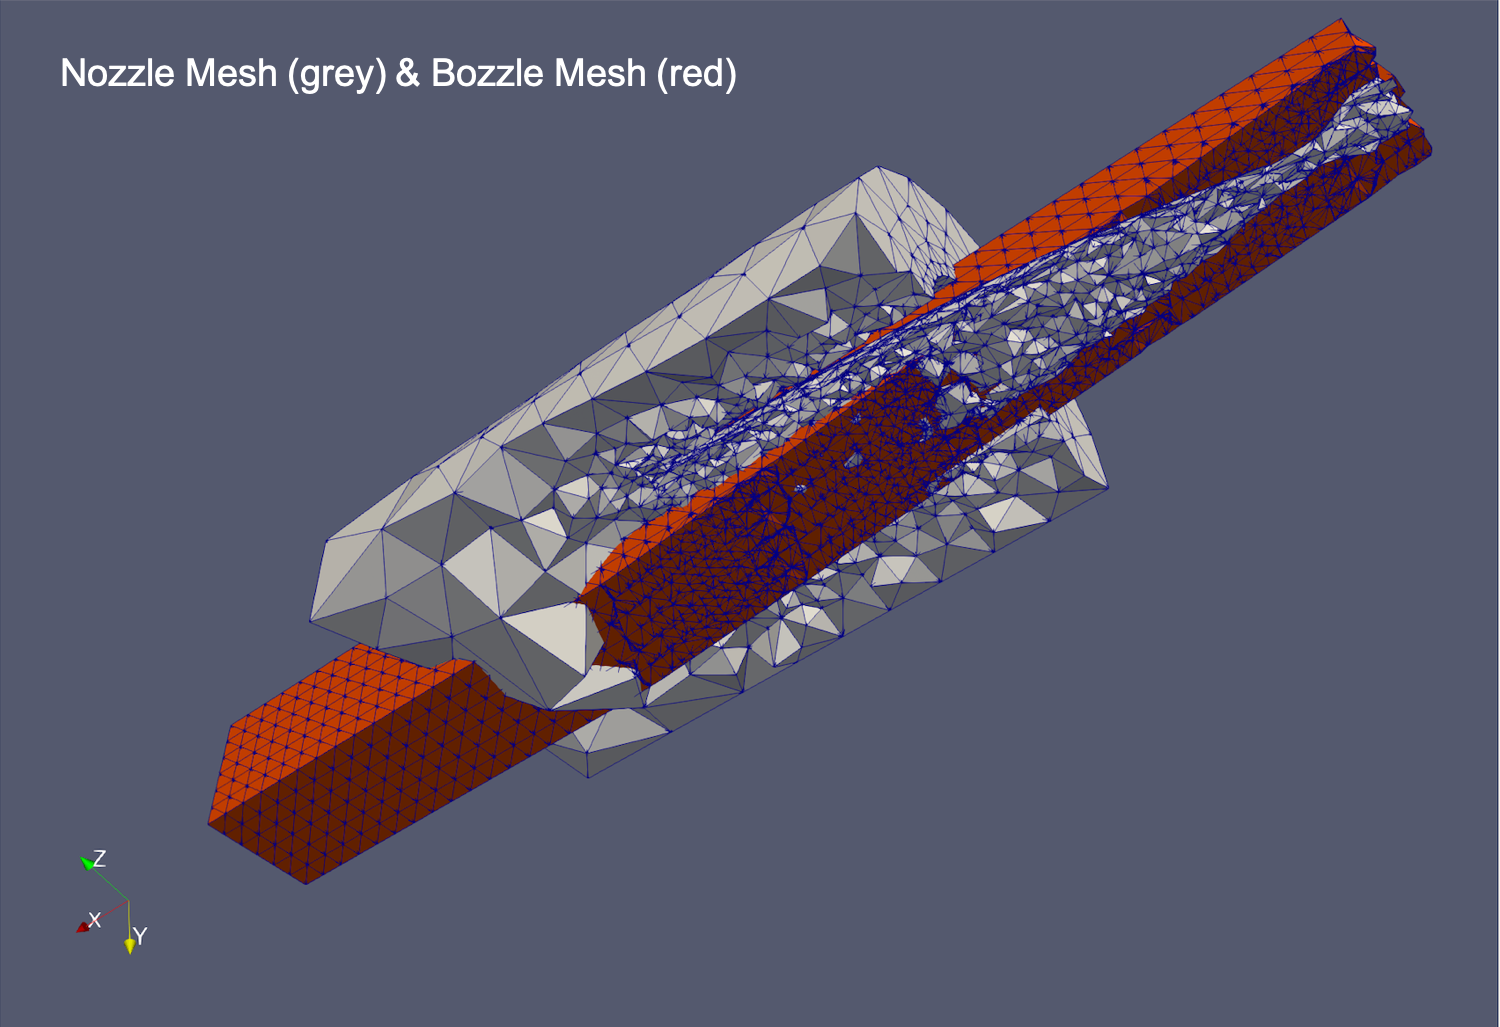
\includegraphics[width=\textwidth]{figures/bono2.png} \\
      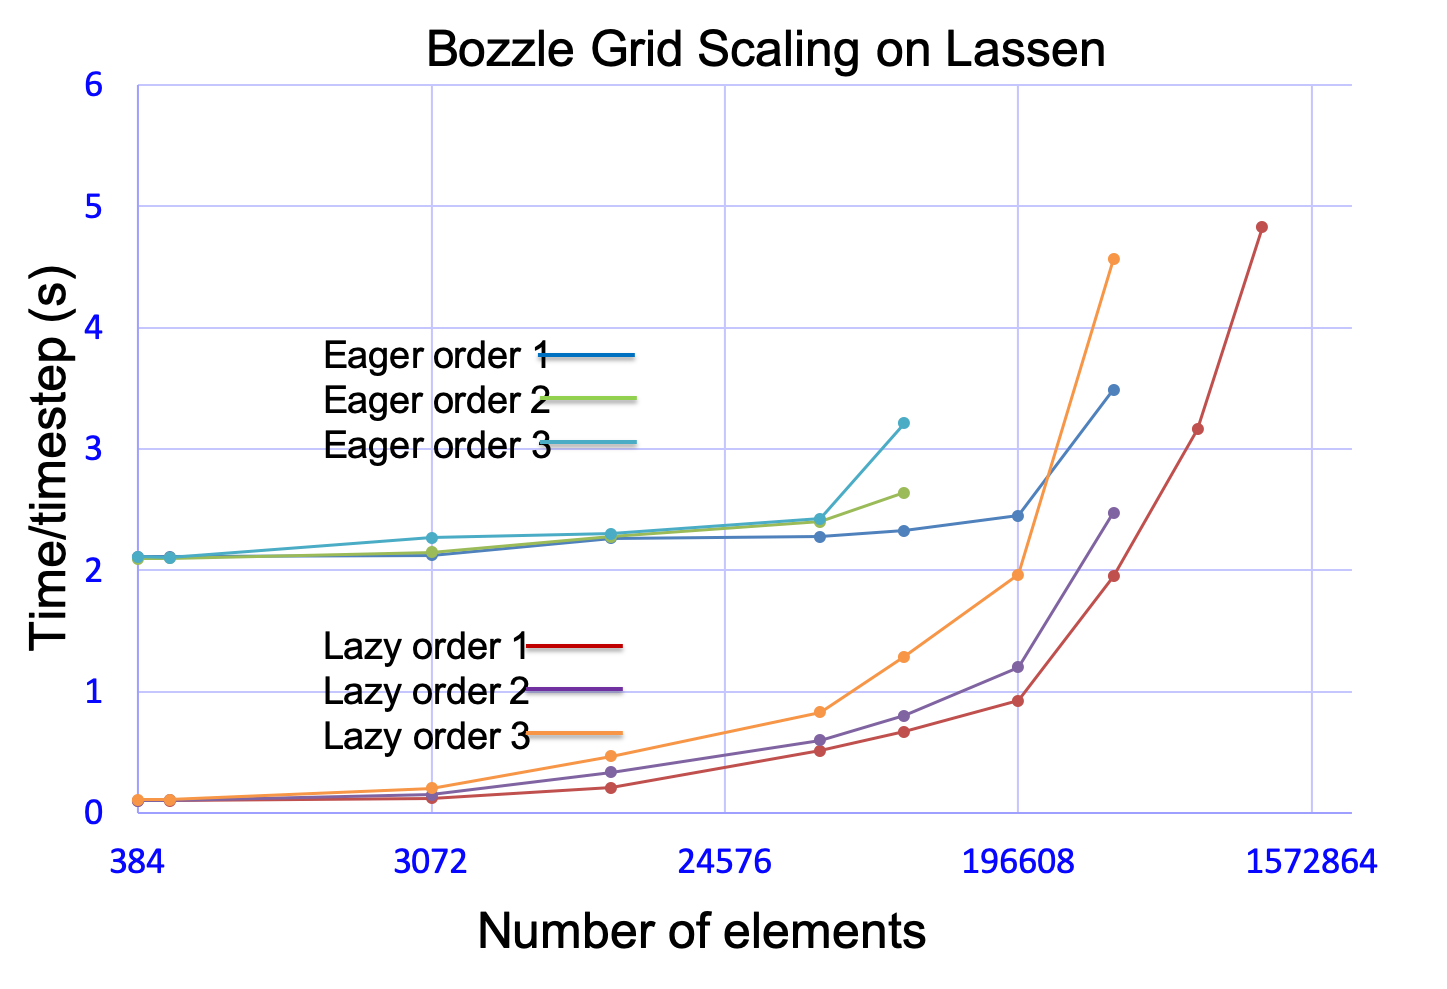
\includegraphics[width=\textwidth]{figures/bozzle_gridscale.png}
    \end{figure}		
  \end{minipage}
\end{frame}

%\begin{frame}\frametitle{Production timing history}
%  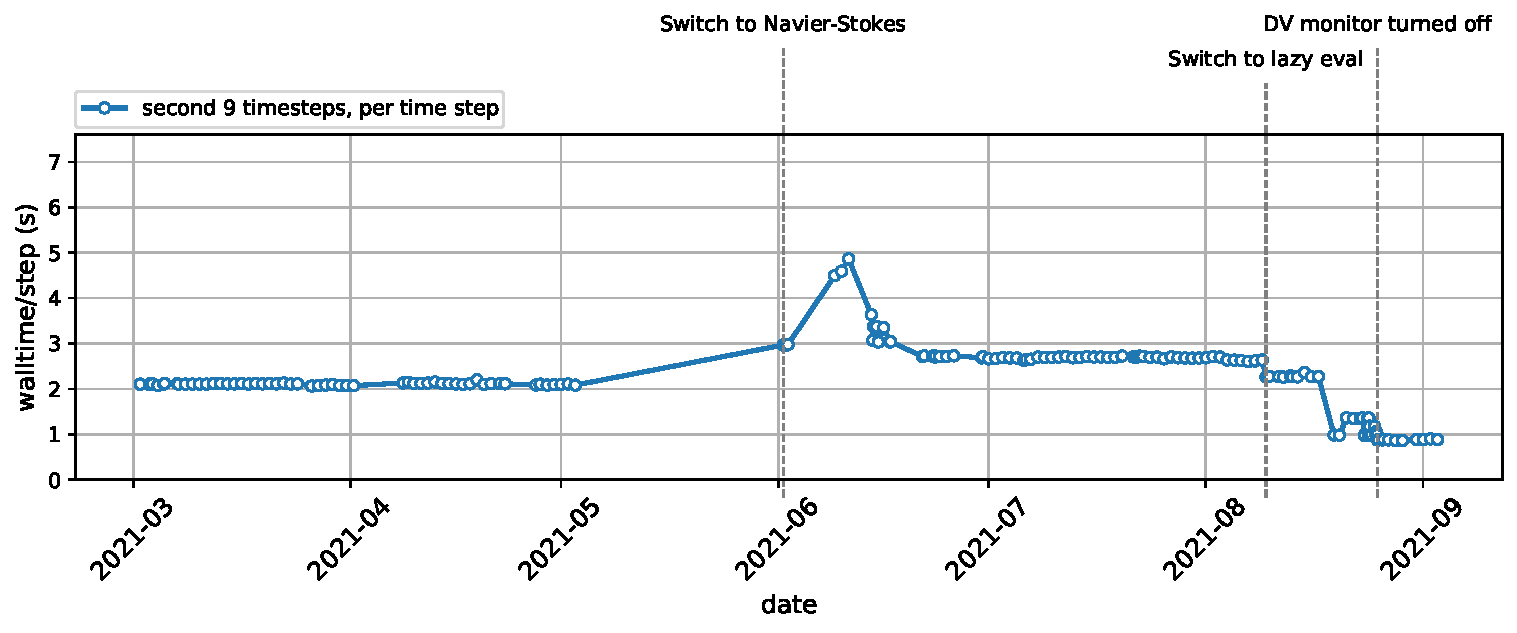
\includegraphics[width=\textwidth]{figures/nozzle_timing.pdf} 
%\end{frame}

%\begin{frame}\frametitle{Conclusion and wrap-up}
%\end{frame}

\begin{frame}\frametitle{Questions from the review team}
  \begin{itemize}
    \item Question 1: \textcolor{red}{Describe the scaling and performance obtained on full-scale ASC and other supercomputers, including a discussion of any limitations encountered.}
    \begin{itemize}  
    \item Eager-mode \textit{MIRGE-Com} is performance challenged, and non-representative
    \item However, we can use eager to expose potential limitations (Python or \textit{MIRGE-Com}) 
    \end{itemize}
  \end{itemize}
  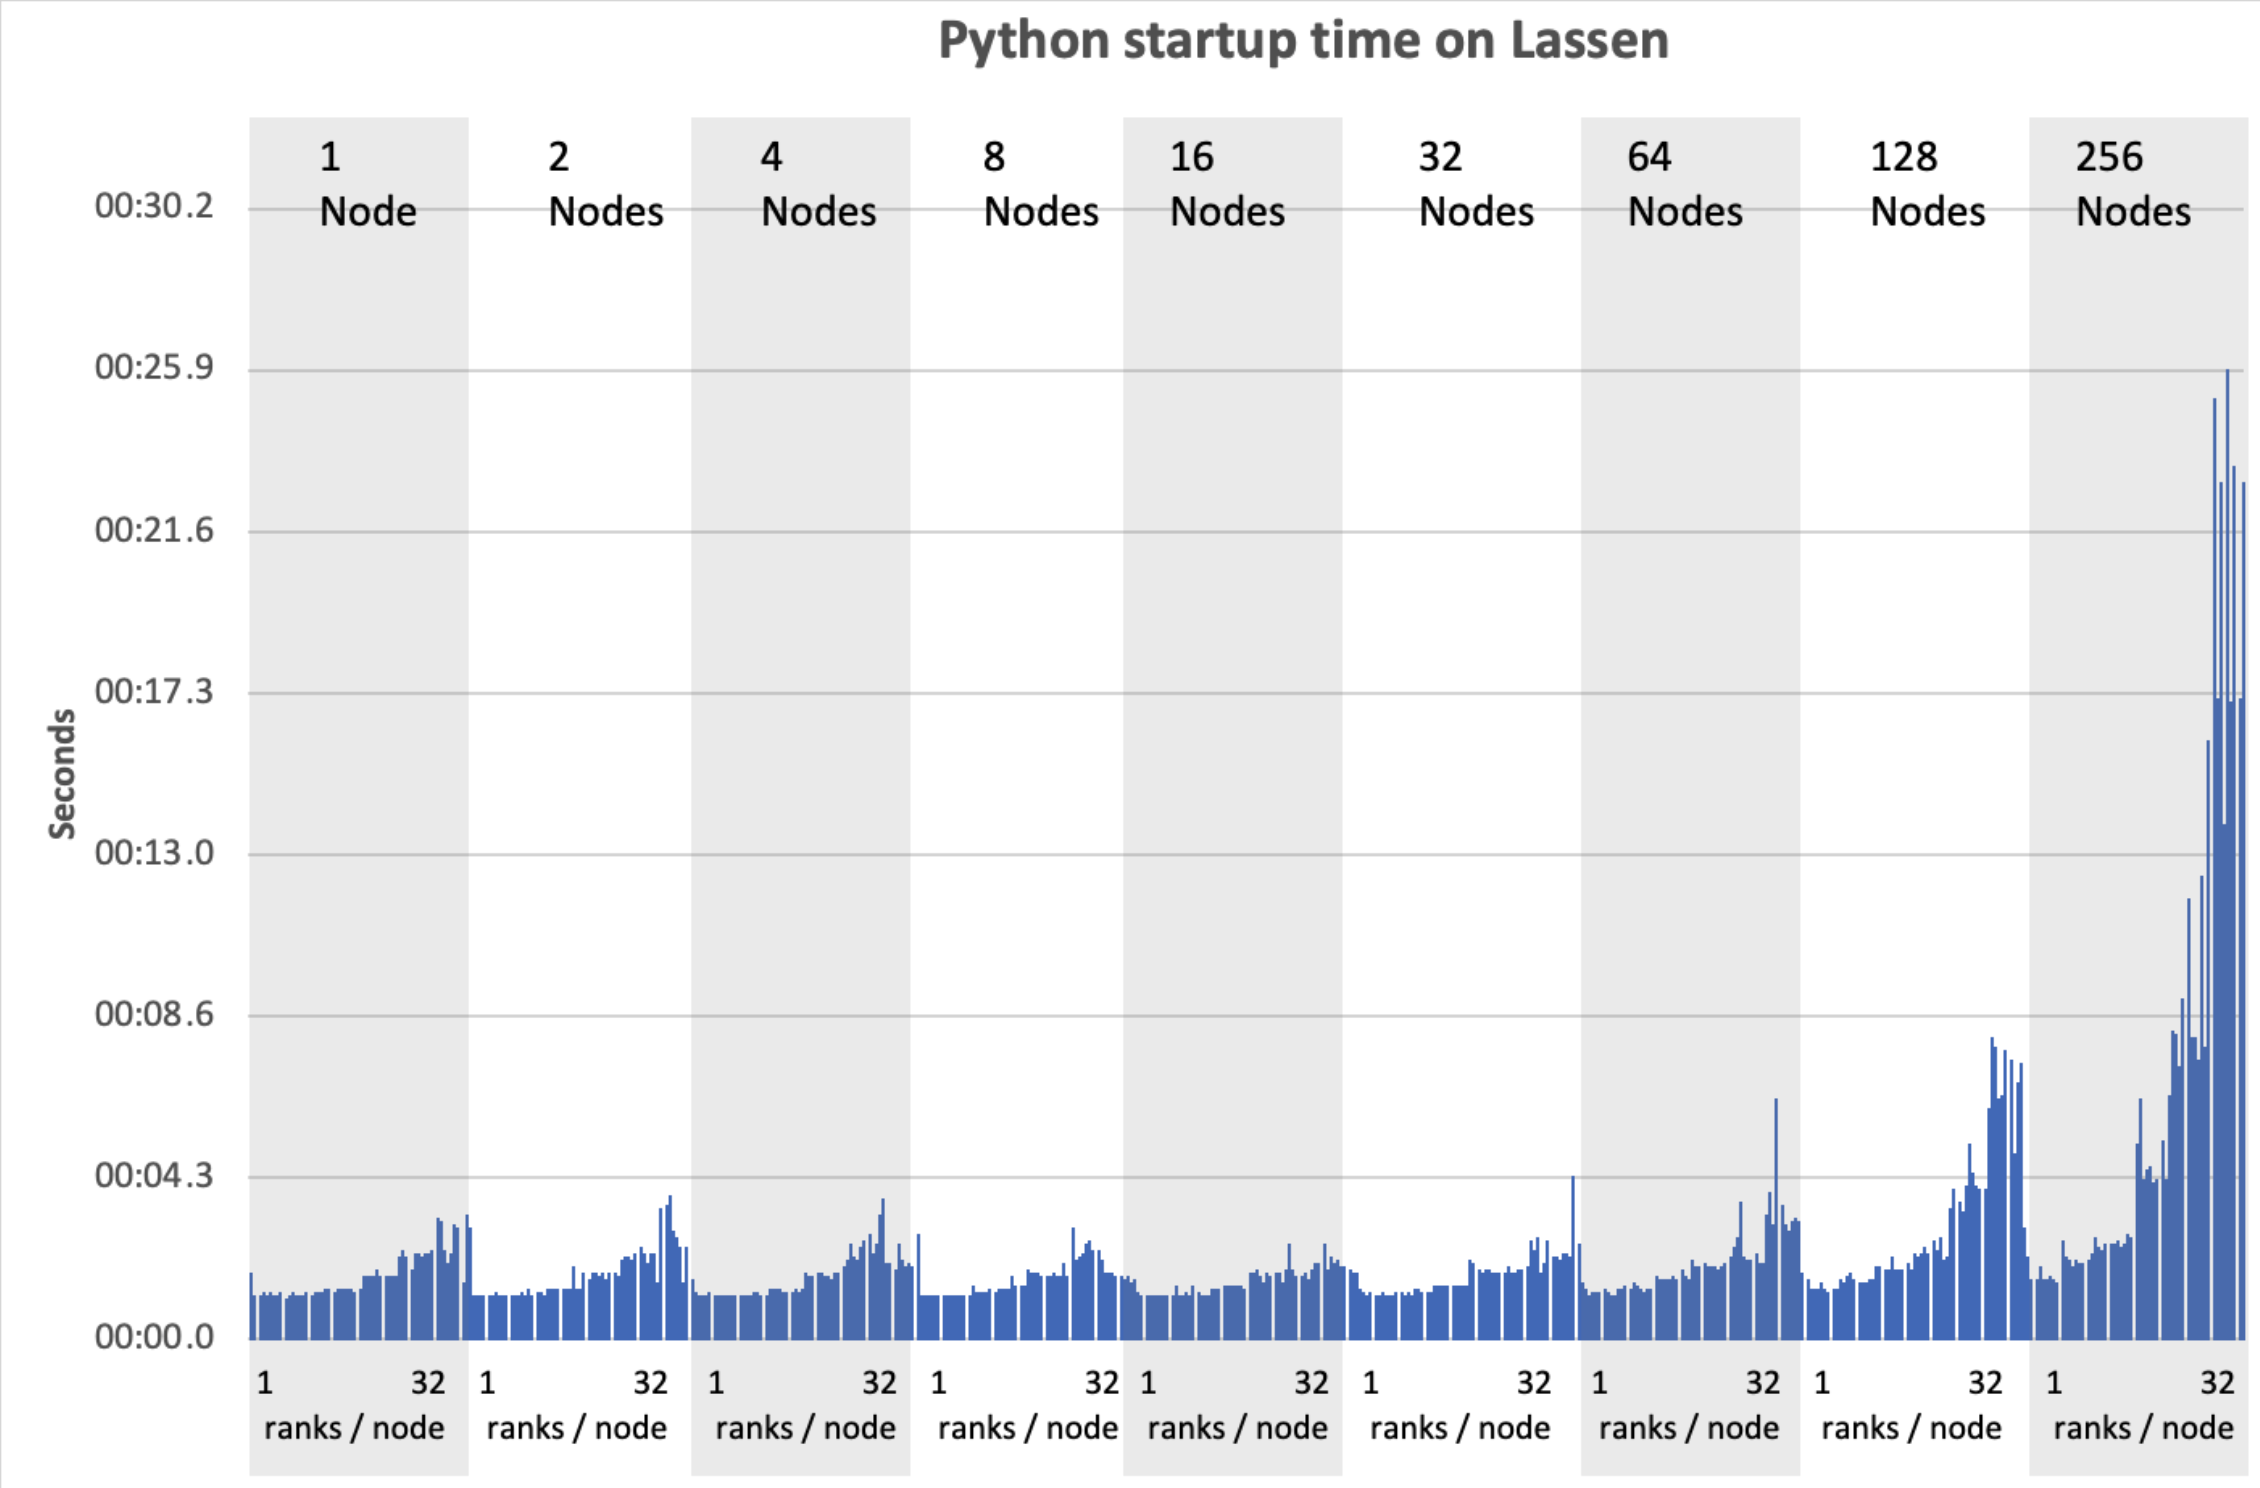
\includegraphics[width=.45\textwidth]{figures/python_at_scale.png}
  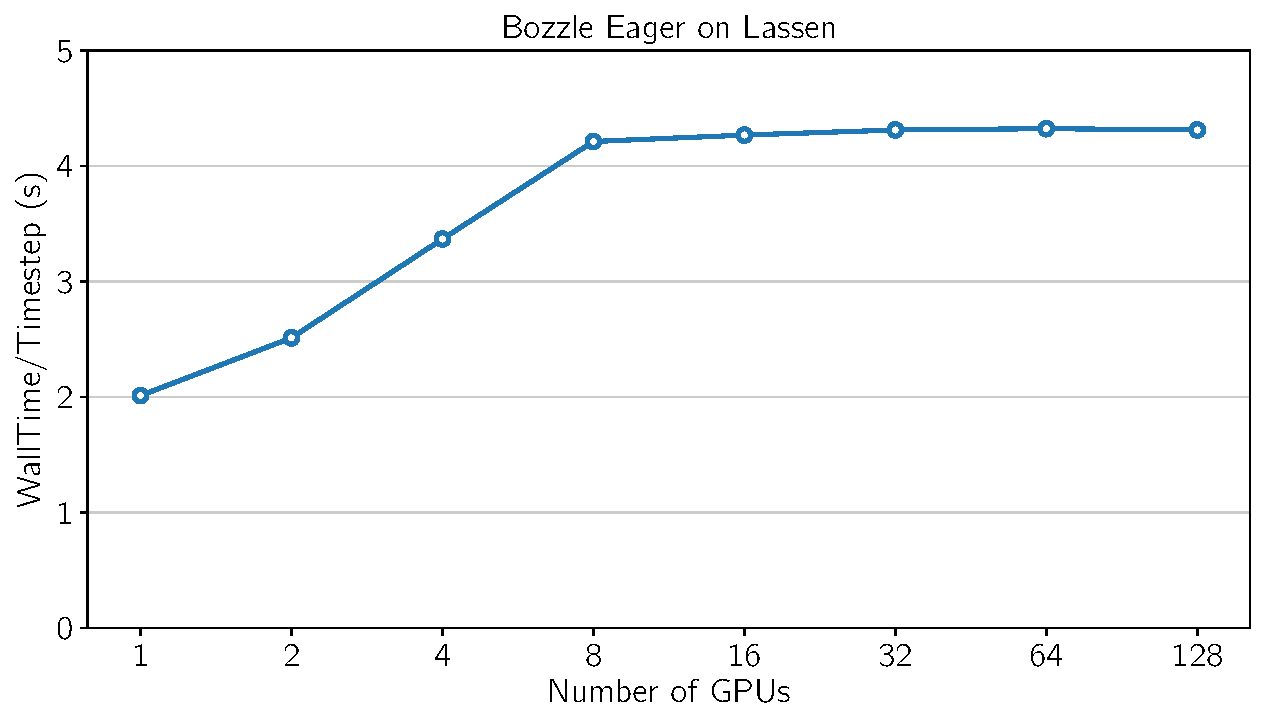
\includegraphics[width=.45\textwidth]{figures/gpuscaling.pdf}
\end{frame}

\begin{frame}\frametitle{Questions from the review team}
  \begin{itemize}
  \item Question 2: \textcolor{red}{Describe the impact of your computer science work on the scaling, portability, and/or programmability achieved.}
    \begin{itemize}
    \item Programmability is great and getting better
      \begin{itemize}
      \item Easy to go from concept/model to working sim application
      \item Quite easy to read and understand 
      \item Close to the symbolic expressions
      \item Improving: Profiling and debugging support, data structures
      \end{itemize}
    \item Portability is OK (does run MPI, threads, OpenCL, CPU/GPU)
      \begin{itemize}
      \item Code readily executes on most platforms
      \item \textit{Emirge} installation utility is (mostly) platform-agnostic
      \item TPLs are the main issue here (e.g. \textit{gmsh}, \textit{Cantera}, \textit{PyOpenCL})
      \end{itemize}
    \item Scalability:
      \begin{itemize}
      \item previously limited to $< 32$ ranks 
      \item Addressed some ballooning startup times
      \item Found and eliminated non-local caches on expensive filesystems
      \item Learning how to plan our production runs: weak scale to lots of DOFs
      \end{itemize}
    \end{itemize}
  \end{itemize}
\end{frame}

\begin{frame}\frametitle{Questions from the review team}
  \begin{itemize}
    \item Question 3: \textcolor{red}{How have you verified and validated \prj{\tiny}{Freund, 05} your simulations?}
  \end{itemize}
  \begin{multicols}{2}
    \begin{itemize}
    \item Integrated verification cases:
      \begin{itemize}
      \item Isentropic vortex % (inviscid terms, exact BCs)
      \item Scalar advection % (inviscid terms, passive scalar components)
      \item Planar Poiseuille % (viscous terms, No-slip, inflow, outflow)
      \item 1DFlame \prj{\tiny}{M.~Anderson} % Autoignition % (chemistry source terms)
      \item Sod's shock \prj{\tiny}{T.~Gibson}  % (demonstrates fail, filtering)
      \end{itemize}
      \columnbreak
    \item Autoignition co-verification
      \begin{itemize}
      \item Ethylene/air mixture $(1500\mathtt{K}, \rho=\mathtt{const})$
      \item \textit{Prometheus}-predicted profiles match \textit{Cantera}
      \end{itemize}
    \end{itemize}
  \end{multicols}
  \begin{multicols}{2}
    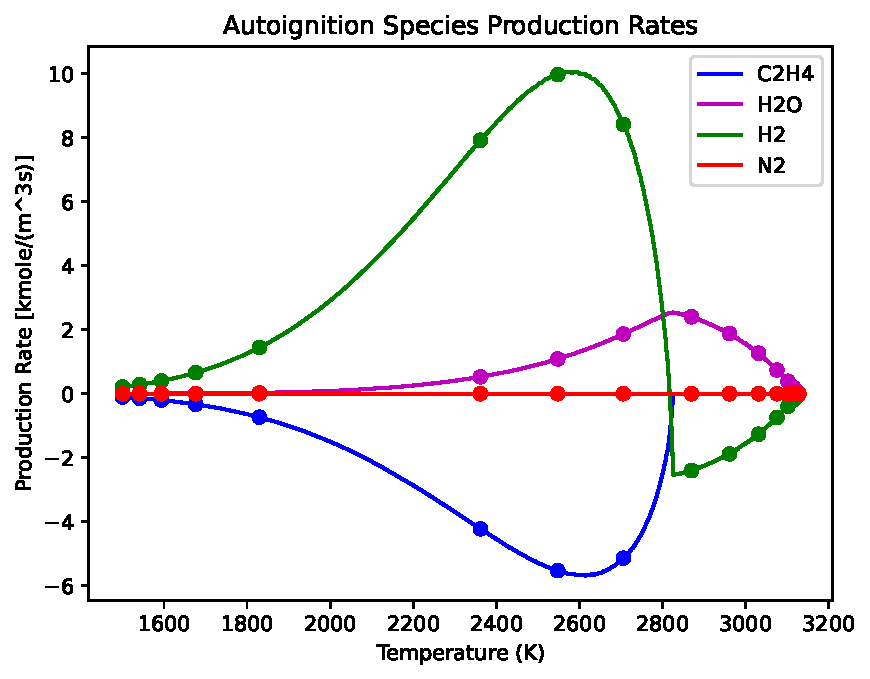
\includegraphics[width=.45\textwidth]{figures/autoignition_rates.pdf}\\
    \columnbreak
    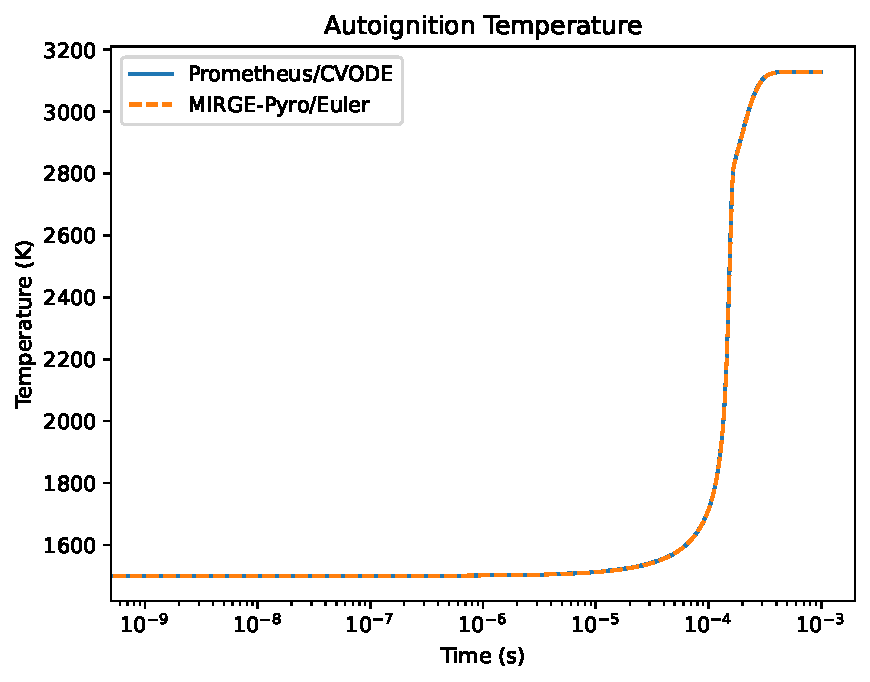
\includegraphics[width=.45\textwidth]{figures/autoignition_temperature.pdf}
  \end{multicols}
\end{frame}

%======================================================================
%\begin{frame}\frametitle{MIRGECom status and developments}
%  \begin{center}
%    Outline
%  \end{center}
%  \begin{itemize}
%  % MIRGE (Com) and how it is constructed, how it comes together
%  \item High-level architecture
%    
%  \item Navier-Stokes w/mixtures \& wall cartoon
%    \begin{itemize}
%    \item highlight current \& to come (Wyatt - shock capt, MattS - wall model, Esteban - thermochem kinetics)
%    \item show example code expressions for NS
%    % How prometheus connects
%    \item show \pyrometheus integration plan (and how is currently implemented)
%    \end{itemize}
%  \item MIRGE-Euler example(s):
%    \begin{itemize}
%    \item Building a driver
%    \item Brief about I/O \& analysis (maybe in arch overview?)
%    \item Autoignition example 
%    \item Allude to MikeA's Y0 sim
%    \end{itemize}
%  \end{itemize}
%\end{frame}
%======================================================================

%\begin{frame}\frametitle{Core packages}
%\begin{itemize}
%  \item Loo.py (\href{https://github.com/inducer/loopy}{(\textcolor{blue}{https://github.com/inducer/loopy})})
%  \begin{itemize}
%    \item Code generator and transform tool
%    \item IR in MIRGE
%    \item Element-wise computational kernels
%  \end{itemize}
%  \item Meshmode (\href{https://github.com/inducer/meshmode}{(\textcolor{blue}{https://github.com/inducer/meshmode})})
%  \begin{itemize}
%    \item Uns., high-order, discont. piecewise polynomial discretizations 
%    \item DG building blocks (see \texttt{examples/simple-dg.py}).
%  \end{itemize}
%  \item \textit{Grudge} - 1/2/3D DG based on \textit{meshmode} (\href{https://github.com/inducer/grudge}{(\textcolor{blue}{https://github.com/inducer/grudge})})
%  \begin{itemize}
%    \item Multiple \textit{meshmode} discretizations
%    \item Methods and operations - math, projections, norms and reductions
%  \end{itemize}
%\end{itemize}
%\end{frame}

%\begin{frame}\frametitle{Development team}
%\begin{multicols}{2}
%\begin{itemize}
%\item Mike Anderson - predictions, modeling
%\item Mike Campbell - sim/solver development
%\columnbreak
%\item Matthias Diener - environment, platforms, performance
%\item Matt Smith  - sim/solver development, grids/geometry
%\end{itemize}
%\end{multicols}
%\end{frame}

%\begin{frame}\frametitle{Target problem}
%  \begin{itemize}
%  \item Domain cartoon
%    % MIRGE (Com) and how it is constructed, how it comes together
%  \item Navier-Stokes w/mixtures \& chemical sources for fluid \& wall cartoon
%  \item Wall and viscous fluxes - Matt Smith heat eqn solver
%  \item Inviscid part - expressions for fluxes, implementation
%  \item Chemistry, \pyrometheus - Esteban
%    \begin{itemize}
%    \item architecture plug here \& generator use to generate python
%    \item expression for sources, implementation
%    \end{itemize}
%  \item Shock-capturing - Wyatt Hagen
%  \end{itemize}
%\end{frame}

%\begin{frame}\frametitle{User experience}
%  \begin{itemize}
%  \item Problem setup
%    \begin{itemize}
%    \item Grid - generate or read in (M. Smith hook)
%    \item Building a driver
%    \item Brief about I/O \& analysis (maybe in arch overview?)
%    \end{itemize}
%  \item Example drivers
%    \begin{itemize}
%    \item Isentropic vortex verif
%    \item Autoignition example 
%    \item Allude to MikeA's Y0 sim
%    \end{itemize}
%  \end{itemize}
%\end{frame}

%\begin{frame}\frametitle{High-level architecture}
%\end{frame}

%\begin{frame}\frametitle{Getting started with \textit{MIRGE-Com}}
%\begin{multicols}{2}
%\begin{itemize}
%  \item \textit{Emirge} - \textit{MIRGE-Com} installation tool
%  \begin{itemize}
%    \item > git clone https://github.com/illinois-ceesd/emirge
%    \item > install.sh
%    \item > source config/activate\_env.sh
%  \end{itemize}
%  \item \textit{MIRGE-Com} documentation
%  \begin{itemize}
%    \item > conda install sphinx
%    \item > cd mirgecom/doc \&\& make html
%  \end{itemize}
%\end{itemize}
%%\hspace{.8in}
%%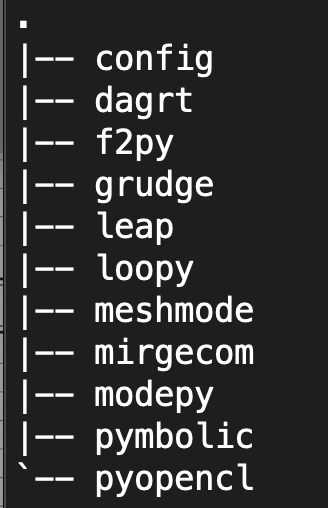
\includegraphics[width=.2\textwidth]{figures/mtc/emirge_dirs.png}
%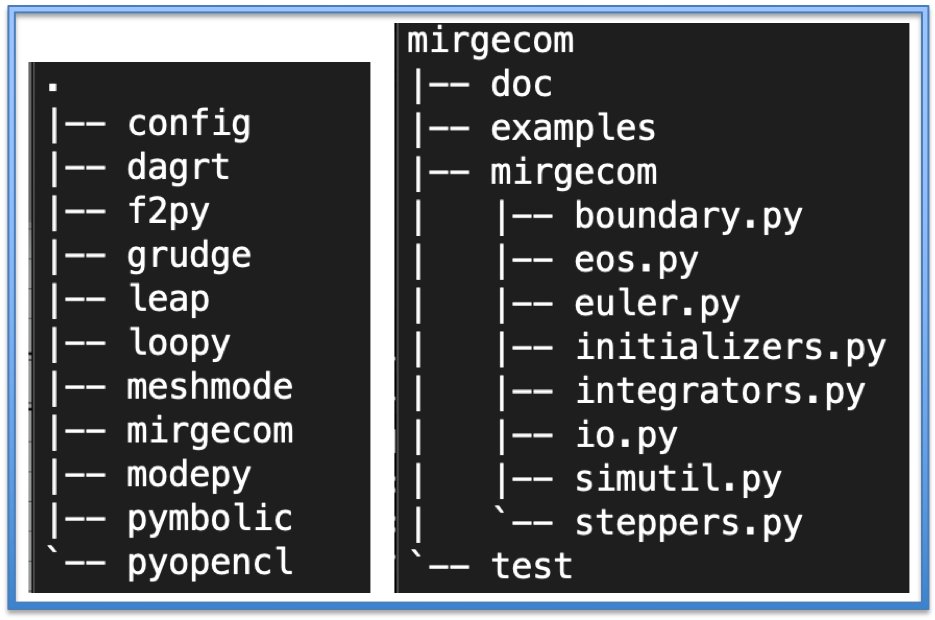
\includegraphics[width=.5\textwidth]{figures/mtc/dir_trees.png}
%\end{multicols}
%\begin{center}
%\href{https://github.com/illinois-ceesd/emirge}{(\textcolor{blue}{https://github.com/illinois-ceesd/emirge})}
%\href{https://mirgecom.readthedocs.io/en/latest/}{(\textcolor{blue}{https://mirgecom.readthedocs.io/en/latest/})}
%\end{center}
%\end{frame}


%\begin{frame}\frametitle{DG Support - Sub-discretizations (dd)}
%  \begin{multicols}{2}
%    \begin{itemize}
%    \item Projections between sub-discretizations: ``vol'' $\rightarrow$ ``int\_faces''
%    \end{itemize}
%    \lstinputlisting[style=kkcodestyle, basicstyle=\scriptsize, language=Python]{figures/mtc/project_sample.py}
%    \columnbreak
%    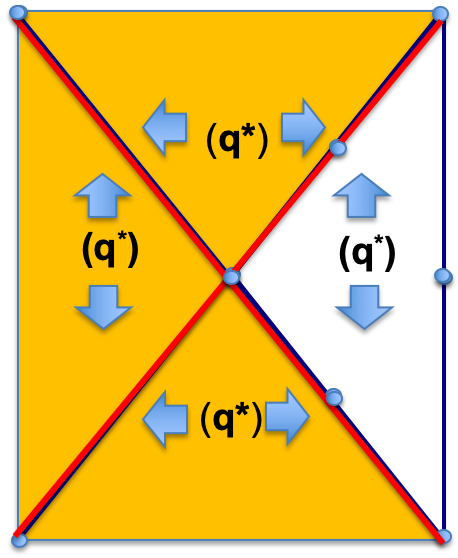
\includegraphics[width=.5\textwidth]{figures/mtc/grid_cartoon_6.png}
%  \end{multicols}
%\end{frame}

%\begin{frame}\frametitle{DG Support - Sub-discretizations (dd)}
%  \begin{multicols}{2}
%    \begin{itemize}
%    \item Unit normal to sub-discretizations
%    \end{itemize}
%    \lstinputlisting[style=kkcodestyle, basicstyle=\scriptsize, language=Python]{figures/mtc/normal_sample.py}
%    \columnbreak
%    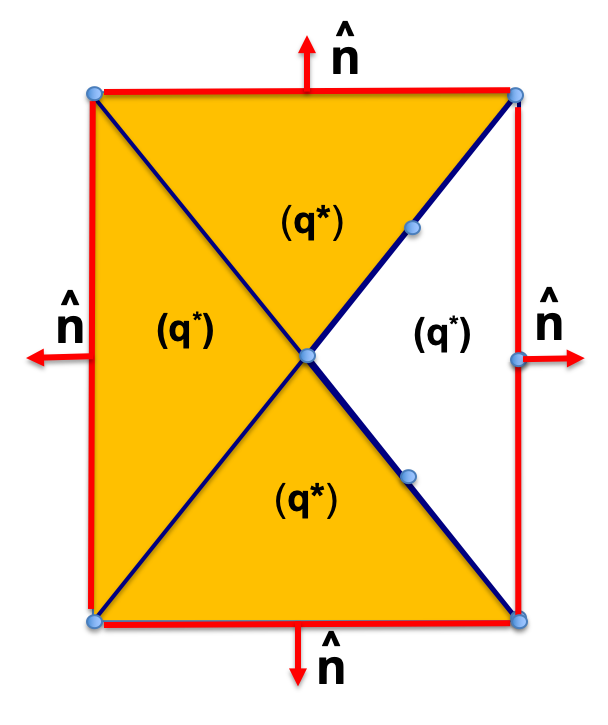
\includegraphics[width=.5\textwidth]{figures/mtc/grid_cartoon_normals.png}
%    %    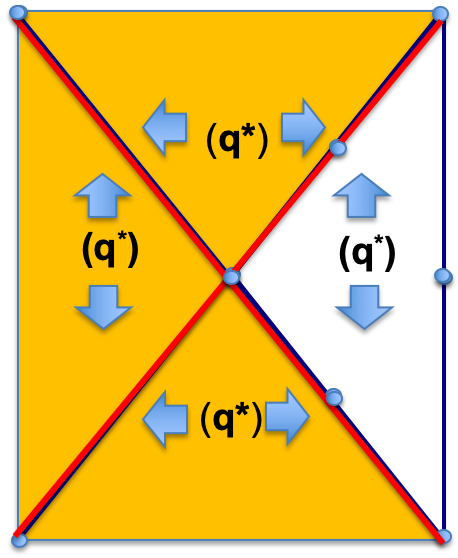
\includegraphics[width=.5\textwidth]{figures/mtc/grid_cartoon_6.png}
%  \end{multicols}
%\end{frame}

%\begin{frame}\frametitle{DG Support - Sub-discretizations (dd)}
%  \begin{multicols}{2}
%    \begin{itemize}
%    \item \textit{Grudge} TracePair data structure for element boundary data
%    \end{itemize}
%% *    \inputminted[mathescape,xleftmargin=0.2in]{python}{figures/mtc/tracepair_sample.py}
%    \columnbreak
%    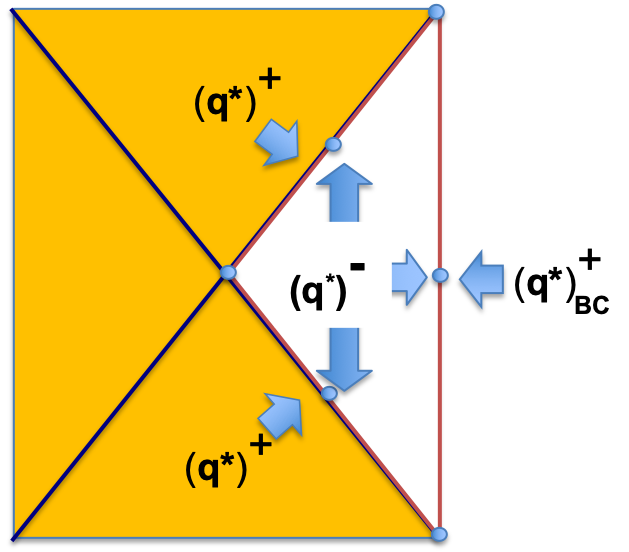
\includegraphics[width=.5\textwidth]{figures/mtc/tracepair_data_cartoon.png}
%  \end{multicols}
%\end{frame}

%\begin{frame}\frametitle{DG Support - Sub-discretizations (dd)}
%  \begin{multicols}{2}
%    \begin{itemize}
%    \item Projections between sub-discretizations: ``vol'' $\rightarrow$ ``int\_faces''
%    \end{itemize}
%    \begin{minted}{python}
%      discr.project("vol", "all_faces", q) 
%    \end{minted}
%    \begin{itemize}
%    \end{itemize}
%    
%    \columnbreak
%    %    %\begin{center}
%    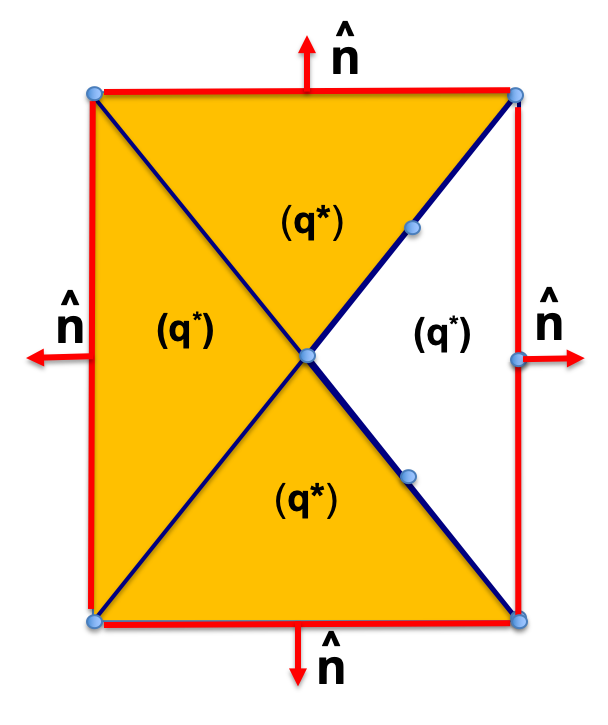
\includegraphics[width=.5\textwidth]{figures/mtc/grid_cartoon_normals.png}
%%    %\end{center}
%  \end{multicols}
%\end{frame}

%\begin{frame}\frametitle{DG Support}
% \begin{multicols}{2}
%\begin{center}
%  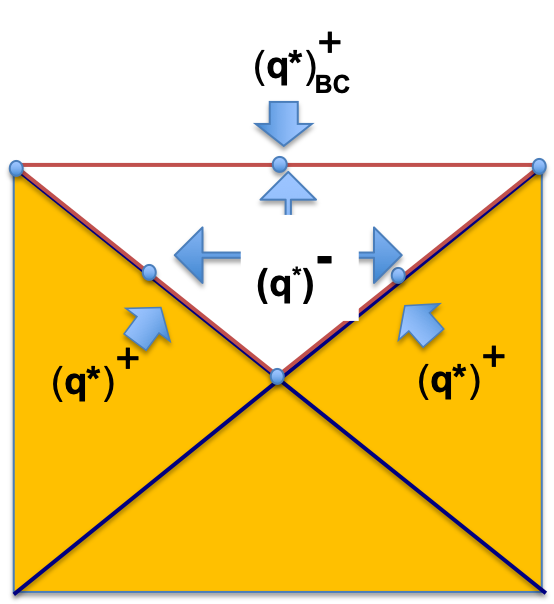
\includegraphics[width=.5\textwidth]{figures/mtc/tracepair_boundaries.png}
%\end{center}
%\end{multicols}
%\end{frame}

% CONS
% Datastructures are a little tough to figure out
% Python - and how it acts on the data structures
% Running afoul of the rules is easy - requires experience
% - some deeper documentation is lacking
% - too hard to discover the rules
% Adding your own kernel C/F90 --> MIRGE
% - mysterious
% Scaling and performance are challenging
%
% PROS
% Follow the rules, and everything works great
% - GPUs, MPI, DG
% Very easy to go from concept and model to working simulation
